%%%%%%%%%%%%%%%%%%%%%%%%%%%%%%%%%%%%%%%%%%%%%%%%%%%%%%%%%%%%%%%%%%%%%%%%%%%%%%%%%%%%%%%%%%
\section{Results and Discussion}

%%%%%%%%%%%%%%%%%%%%%%%%%%%%%%%%%%%%%%%%%%%%%
\subsection{Franke Data}
\begin{figure}[H]
    \centering 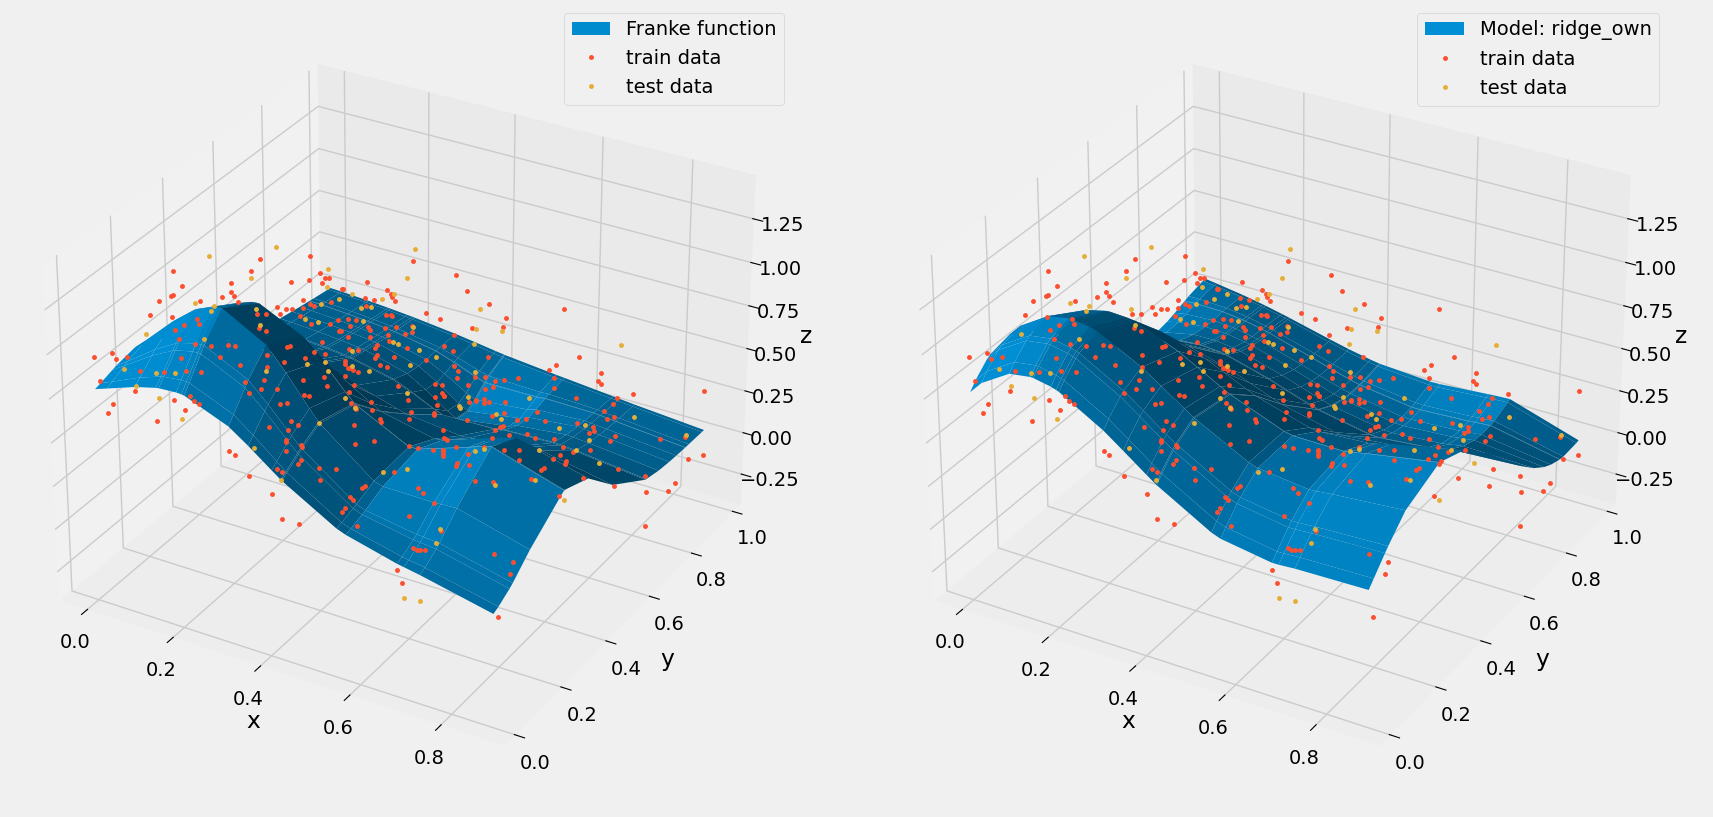
\includegraphics[width=0.8\textwidth]{Figures/franke_data_and_model_ridge_best.png}
    \caption{Left figures shows the frank function plotted as a function of x
    and in y coordinates the intervall [0,1]. The red and yellow dots shows or
train- and test-data with added normal distributed noise, $0.2 \cdot
\sigma(0,1)$. The lowest MSE, calculated with bootstrap re-sampling was obtained
with Ridge regression with a regularization parameter $\lambda = 10^{-5}$ and a
polynomial degree of 5. Right figure shows the best fit model. Train- and
test-data is plotted as for the left figure.} 
\end{figure}

\begin{figure}[H]
     \centering
     \begin{subfigure}[t]{0.49\textwidth}
         \centering
         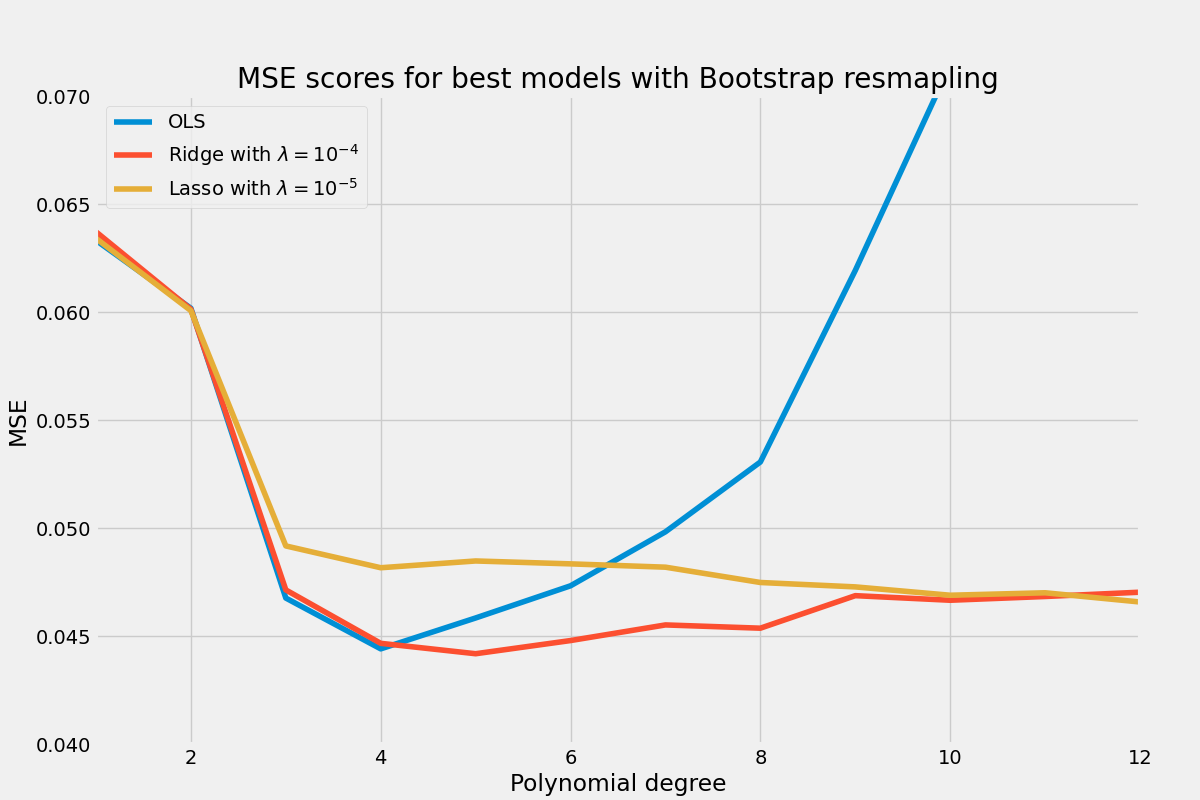
\includegraphics[width=\textwidth]{Figures/franke_ols_ridge_lasso_boots.png}
         \caption{Mean MSE score for 100 bootstrap re-samples. MSE scores is
             plotted as a function of polynomial degree, for the best fit
             models obtained with OLS, Ridge ($\lambda =
             10^{-j}$) and Lasso ($\lambda = 10^{-5}$) regression.}  
         \label{} 
     \end{subfigure}
     \hfill
     \begin{subfigure}[t]{0.49\textwidth}
         \centering
         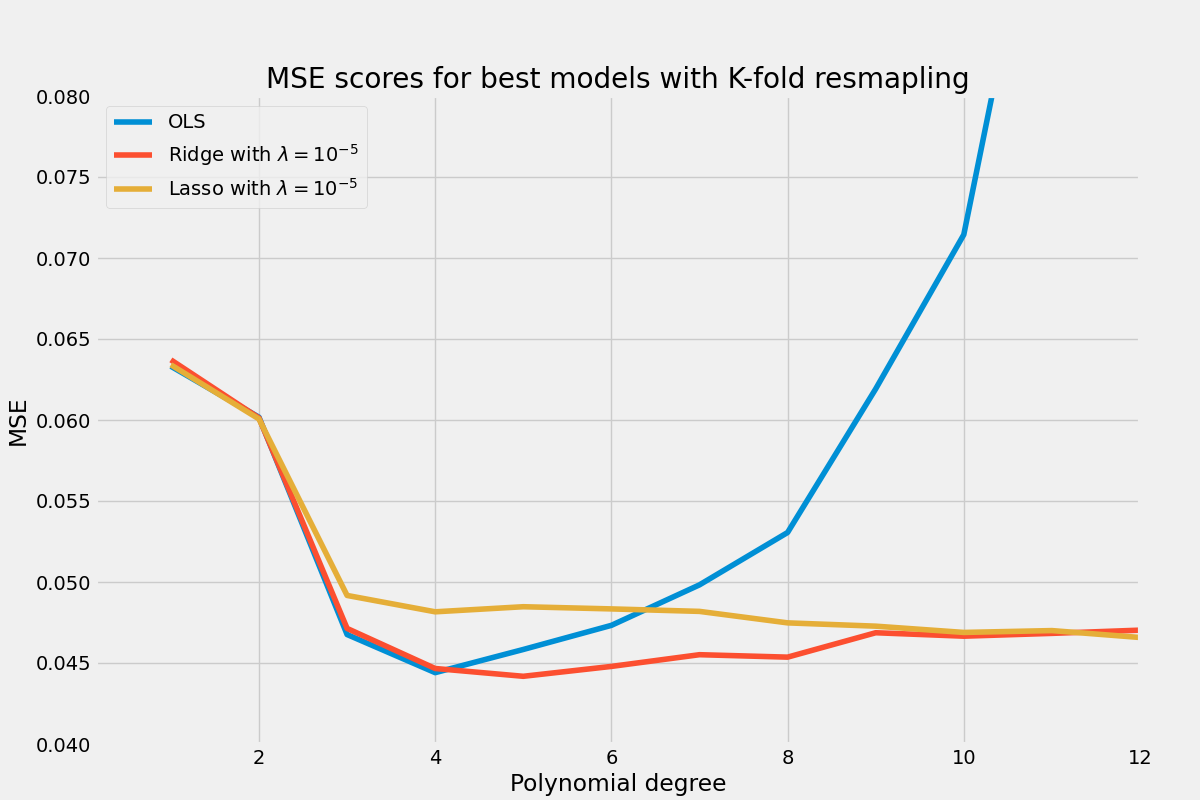
\includegraphics[width=\textwidth]{Figures/franke_ols_ridge_lasso_kfold.png}
         \caption{Mean of MSE scores calculated on all ten test folds with K-fold
             re-sampling. Our best fit models from OLS, Ridge ($\lambda =
             10^{5}$) and Lasso ($10^{-5}$) regression
     is plotted as a function of polynomial degree. $\lambda $ is the 
 regularization parameter.}  
         \label{fig}
     \end{subfigure}

\end{figure}


\begin{table}
    \centering
    \caption{Table of Best mean squared error (MSE) scores obtained with
        different re-sampling and regression
        methods. The training- and testing-data splits from the Franke function
        was used for model fitting and
        prediction respectively. $\lambda $ is the best choice of regularization parameters for
        Ridge and Lasso regression. n refers to number of re-samples/splits used in
        Bootstrap and K-fold.}  
    \label{tab:franke_mse_best} 
    \begin{tabular}{|c|c|c|c|c|}
        \hline
        Polynomial degree & $\lambda$ & Regression method & Re-sampling method & MSE \\
        \hline
                      4    &    & OLS & Bootstrap (n=100) & 0.04440 \\
        \hline
                      5   & $10^{-4}$  & Ridge & Bootstrap (n=100)& 0.04425 \\
        \hline
                      11  & $10^{-5}$  & Lasso & Bootstrap (n=100)& 0.04673 \\
                      
        \hline
                      5    &   & OLS &  K-fold (n=10) &  0.04181\\
        \hline
                      6   &  $10^{-5}$  & Ridge &  K-fold (n=10) & 0.04155 \\
        \hline
                      12  &  $10^{-5}$ & Lasso &  K-fold (n=10) & 0.04548 \\
        \hline
    \end{tabular} 
\end{table}

% TODO OLS scores

%%%%%%%%%%%%%%% Parameters %%%%%%%%%%%%%%%
% n_data = 20 - n_data in x and y: n_tot = 20*20
% test_size = 0.2
% noise = 0.2 - aptitude of normal distributed noise    
% data_dim = 2

%%%%%%%%%%%%%%% Part b %%%%%%%%%%%%%%%
% * Evaluate MSE up to 5.th order fro OLS. 
% * and R2 score
% * blot parameters beta
% * Your code has to include a scaling/centering:
%   XXX: not included, data is already scaled in intervall [0, 1]

\begin{figure}
     \centering
     \begin{subfigure}[b]{0.5\textwidth}
         \centering
         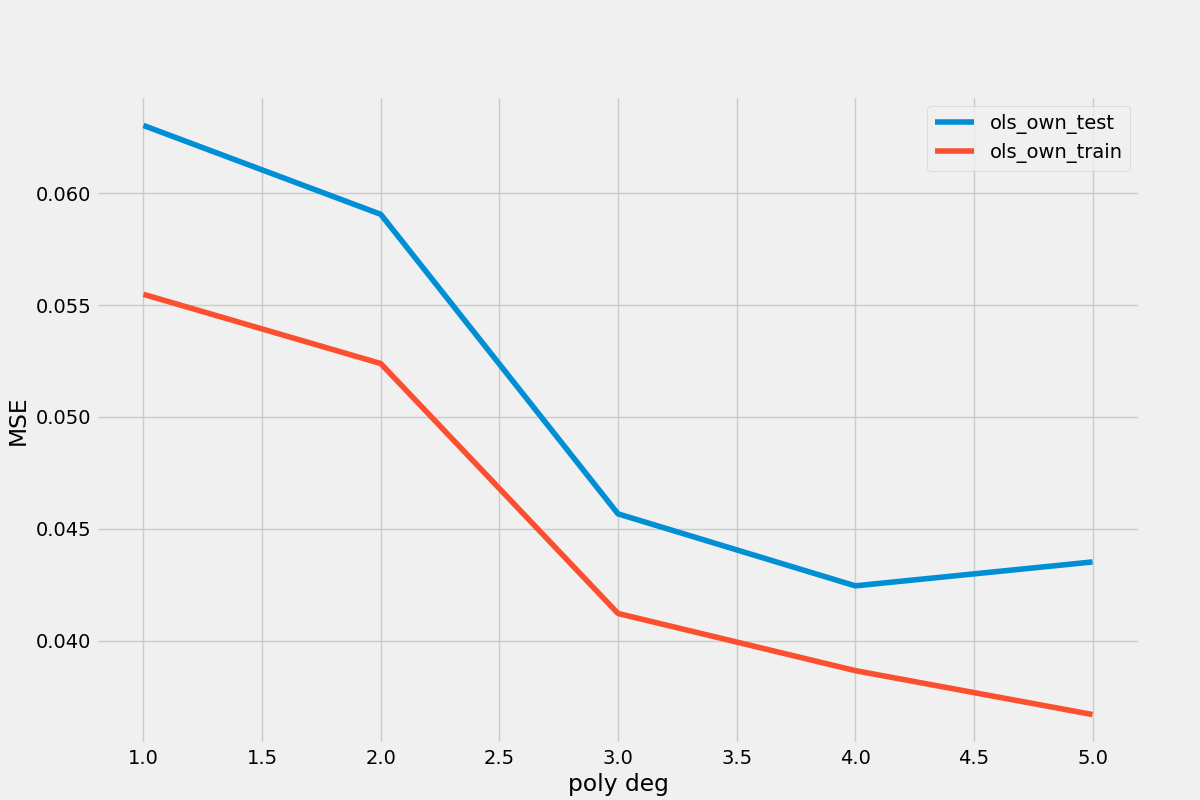
\includegraphics[width=\textwidth]{Figures/b_mse.png}
     \end{subfigure}%
     \hfill
     \begin{subfigure}[b]{0.5\textwidth}
         \centering
         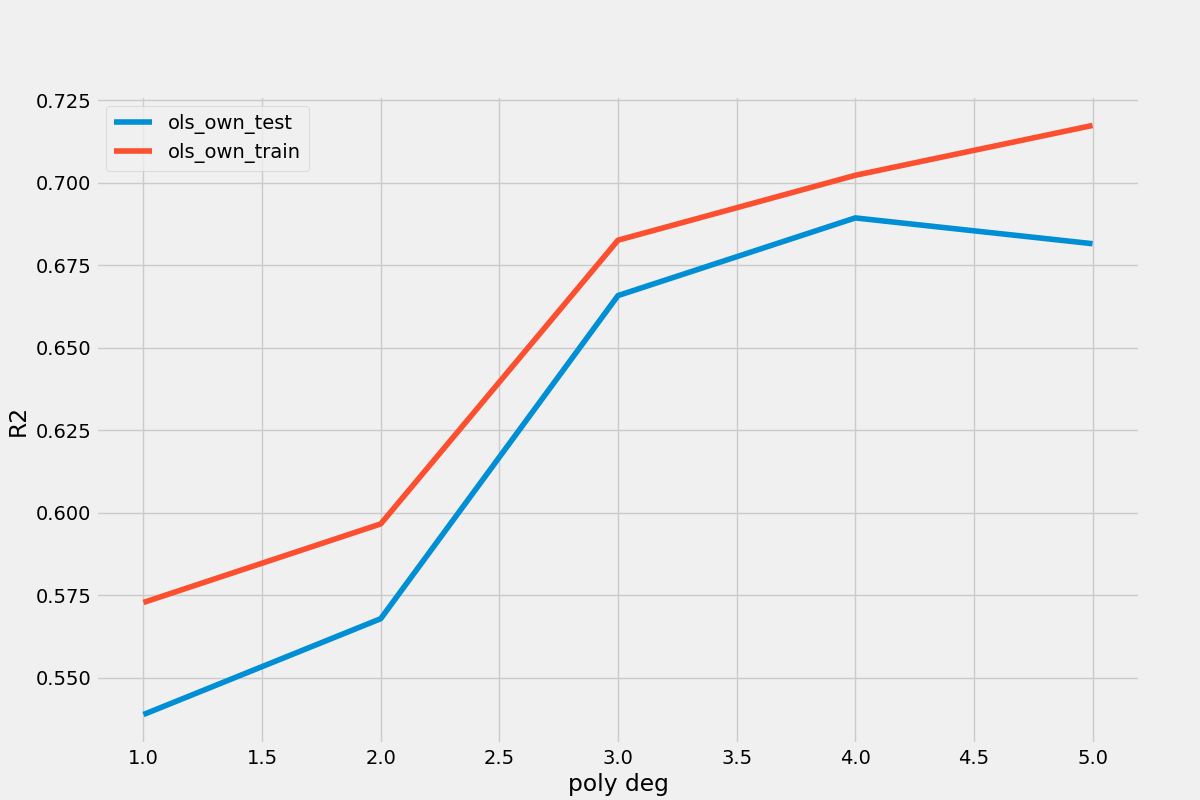
\includegraphics[width=\textwidth]{Figures/b_r2.png}
     \end{subfigure}
        \caption{Mean squared error and score function for the Ordinary Least Squares (OLS) method on the Franke function with N=????? for training and test data with a test/train split of 0.2}
        \label{fig:mse_and_score_franke}
\end{figure}

% Results and discussion of r2 and mse franke plots.  
In figure \ref{fig:mse_and_score_franke} we see the mean squared error and R2
score on the Franke function for a polynomial up to degree five. The Predicted
MSE scores with respect to polynomial degree was predicted on both the training
aand test data. As expected out model gets better as the polynomial degree
increases. That is, our MSE score decreases and R2 score increases. For
polynomial degree 5, the MES score increase for the test data and decreases for
the training data. The opposite behavior is seen for the R2 score. This is an
expected behavior. For increases polynomial degree we should expect that
predictions on the training data gets better and betters, since our model is
trained on the exact same data. Thus, for the prediction on training data we
expect the MES to approach zero as the polynomial degree increases. The same
behaviour can not be expected when we predict MES and R2 score on the test
data. Our model has never seen the test data. We expect that the MES score
predicted on the test data decreases to a certain polynomial degree. Afterward
it will increase, when we have reached over fitting. That is, our model is
fitted to well to the training data, and is no longer generalizable to other
similar distributed datasets. This is the exact behavior we observe in figure
\ref{fig:mse_and_score_franke}. However, the effect if over fit is not
presented very well cause of the low polynomial degree. 

% Scaling - TODO - put in method section? 
If our
predictors represent different scales, then it is important to standardize the
design matrix. 
And as the x and y data is on the same interval $[0, 1]$ we do
not need to scale the data.
% TODO: explain why

%\begin{figure}[H]
%    \centering
%    \caption{Mean square error as function of polynomial degree for }
%    \label{fig:ols_franke}
%    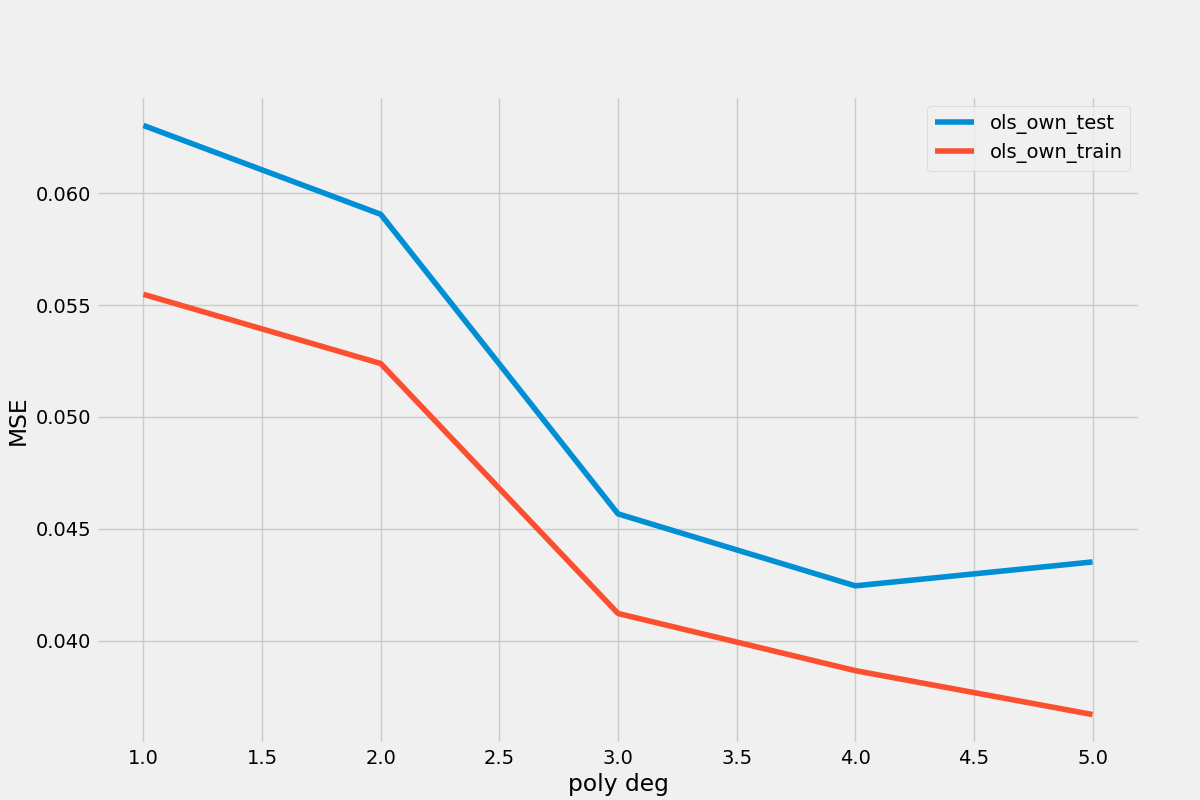
\includegraphics[width=0.8\textwidth]{Figures/b_mse.png}
%\end{figure}

%\begin{figure}[H]
%    \centering
%    \caption{}
%    \label{fig:score_franke}
%    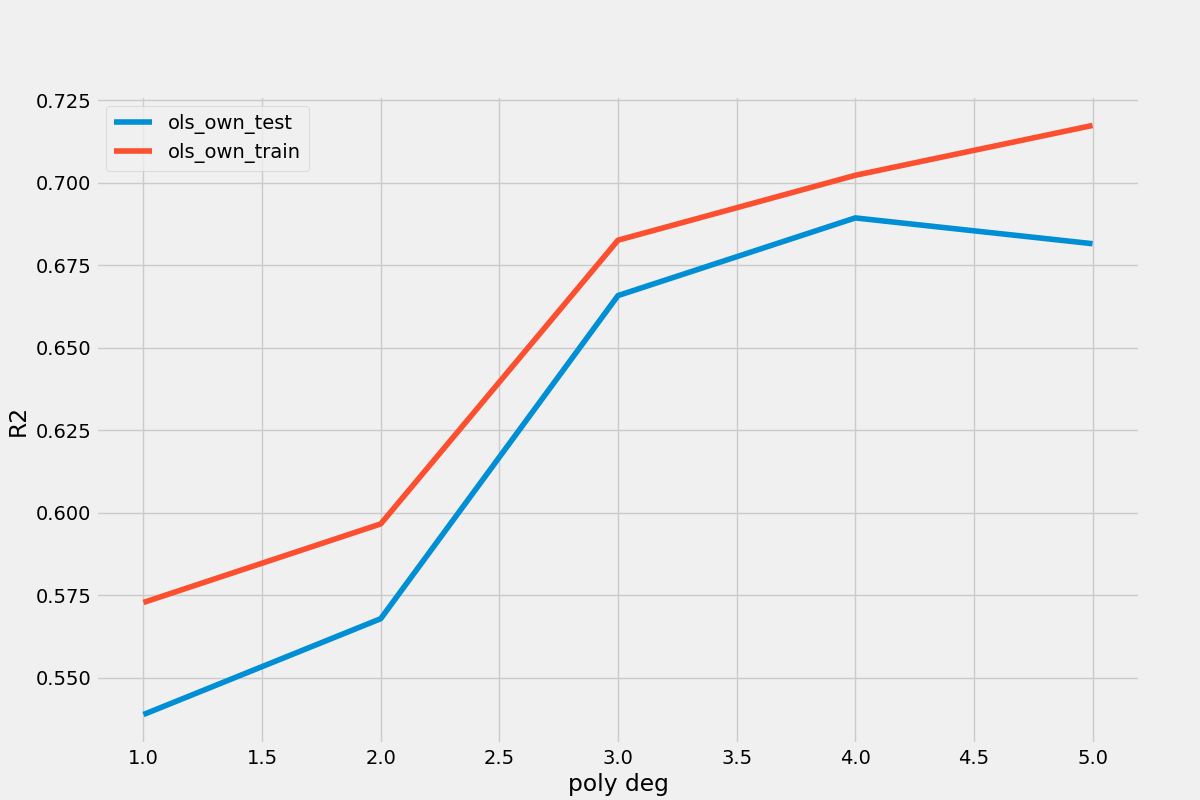
\includegraphics[width=0.8\textwidth]{Figures/b_r2.png}
%\end{figure}

% TODO: error bars
\begin{figure}[H]
    \centering
    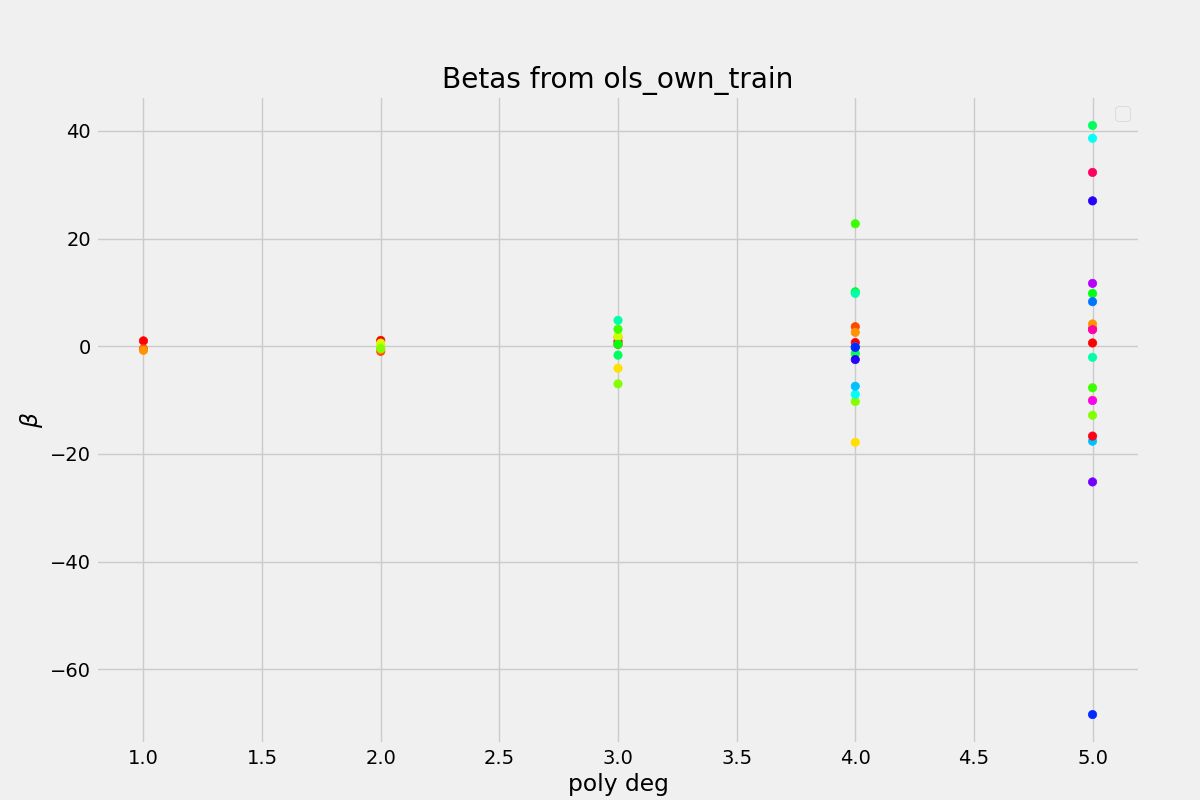
\includegraphics[width=0.8\textwidth]{Figures/b_beta.png}
    \caption{ $\beta _i$ values plotted with respect polynomial degree for our best
    fit model with OLS on the training data, $\bm{X} _{train} $ 
    The colors represent specific $\beta _i$, in order to make it possible to
    track specific $\beta _i$ for different polynomial degrees.      }
    \label{fig:beta_plot}
\end{figure}

% Discussion of beta's
In figure \ref{fig:beta_plot} we see for each polynomial degree the beta
parameters $\beta_i$ as a dot in the plot. This is for the OLS model on the
training data from the Franke function. We see that as the polynomial degree increases, the $\beta$
values deviate more and more from zero. This can be a result of over fitting
since we do not have any regularization parameter on the OLS model.

We expect the different $\beta _i$ does not vary significantly with increasing
polynomial degree. It's not easy to say if this is the case from inspection of
the plot, due to a limited number of colors and large number of $\beta _i$. It seems to be the case for the
lower $\beta _i$ terms. It does not make intuitively sense if a certain $\beta _i$ varies a
lot for different polynomial degree's. The less complex model (lower poly deg) should to a certain degree
reflect the values in a more complex model. By introducing higher polynomials
and hence more $\beta _i$'s, our model can represent more and more complex
patterns (more variations in shorter length scale). However we expect the lower
oerder $\beta _i$ to be more or less the same. Because they represent the less
complex parts of our model. 
 
% TODO: Discuss variance of beta


%For bootstrap: should consider plotting a histogram of the estimators beta_hat^* as this should resemble a pdf. 

%%%%%%%%%%%%%%% Part c  %%%%%%%%%%%%%%%
% * Explain bias, variance, mse terms (theory) and interpretation - XXX: where
% is this done?
% * Bias variance analysis on franke function
% * discuss in bias variance trade-off in terms of:
%   * model complexity
%   * number of data points
%   * training and test data

%%bootstrap figures for different number of datapoints
\begin{figure}
     \centering
     \begin{subfigure}[b]{0.5\textwidth}
         \centering
         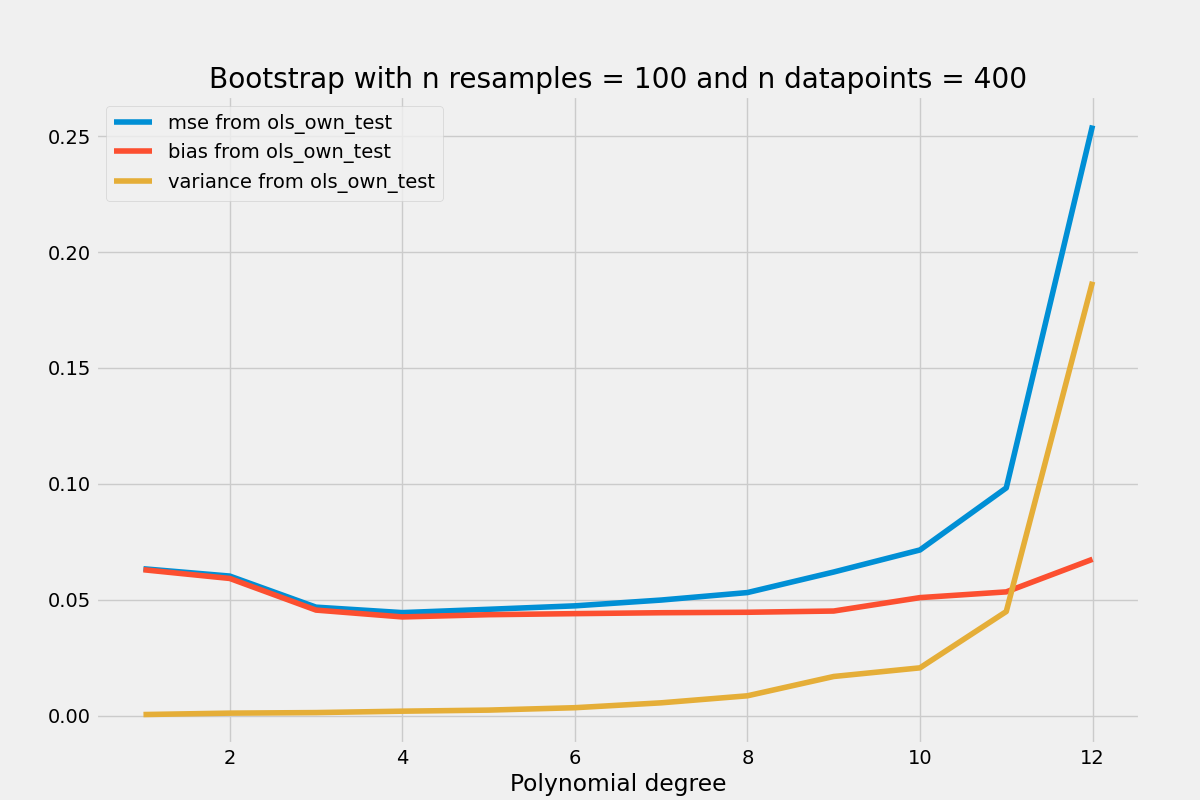
\includegraphics[width=\textwidth]{Figures/c_bootstrap_ols_n_data_400.png}
         \caption{400 datapoints}
     \end{subfigure}%
     \hfill
     \begin{subfigure}[b]{0.5\textwidth}
         \centering
         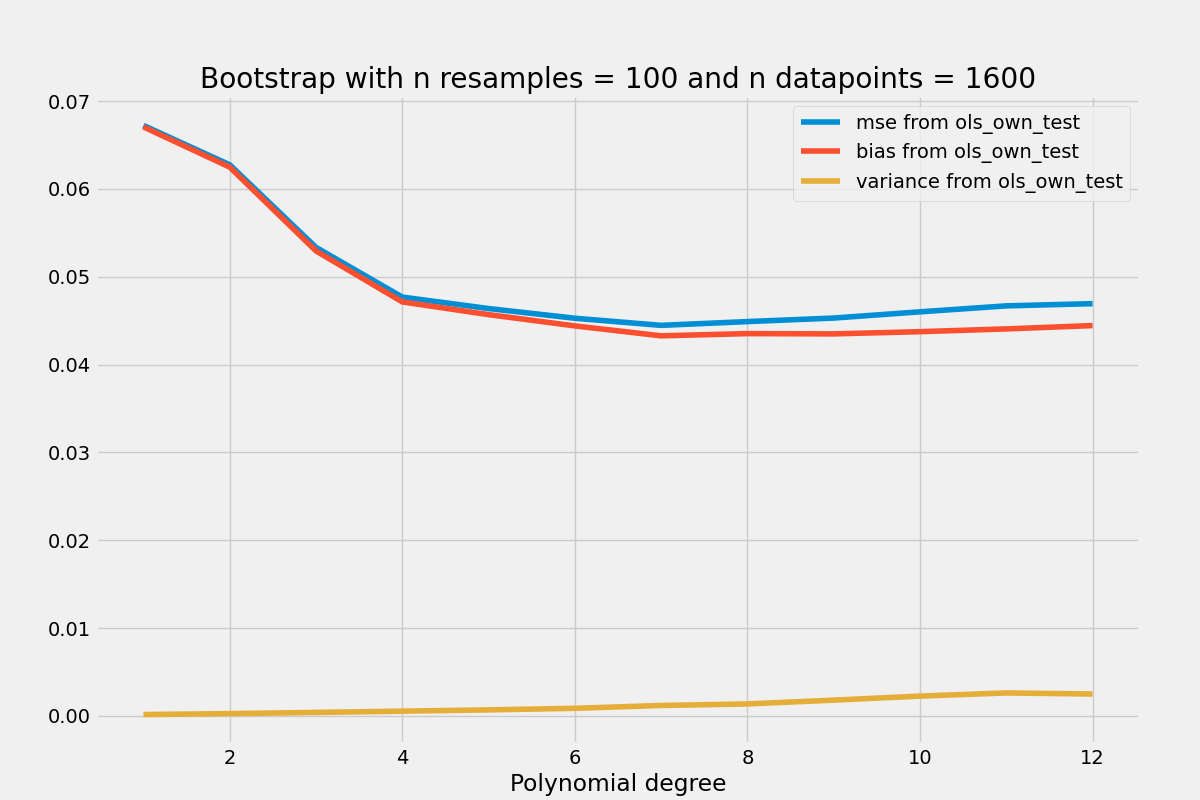
\includegraphics[width=\textwidth]{Figures/c_bootstrap_ols_n_data_1600.png}
         \caption{1600 datapoints}
     \end{subfigure}
        \caption{Bootstrap with 100 resamples for the OLS method on the Franke function on the test set.}
        \label{fig:bootstrap_ols_franke_test}
\end{figure}


In figure \ref{fig:bootstrap_ols_franke_test} we can see the bootstrap used
on the OLS method on the Franke function for 100 resamples and two different
number of datapoints. We see that for the lower number of points we get signs
of overfitting, while we do not see this behaviour at these polynomial degrees
for 1600 datapoints. We see that for 400 datapoints the optimal bias-variance
tradeoff happens at a polynomial degree of around 4 and for 1600 datapoints at
around polynomial degree 7. 

This means that our best fit model is depend the size of the dataset. For
larger dataset sizes the mean value of our data points will resemble more and
more the real distribution. This is also the case for our training data and
test data. To achieve over fit the complexity of the model needs to be very
large.  

In figure \ref{fig:bootstrap_ols_franke_train} the MSE predicted on the training
data with OLS and bootstrap resampling is plotted as function of polynomial
degree. Here we see a similar trend as for the predictions with bootstrap on
the test data. If we had trained the model on the real training data, we would
expect that the predictions of MSE on the training data approaches zero. Our
predicted model should be able to 100\% replicate our data, since the model is
trained the exact same noise. In this scenario it does not make much sense to
talk about over fitting. Cause we need two independent datasets to predict the
generalizability of our model. 

However in our case we did re sample the training dataset (bootstrap with 100
resamples) before we trained our
model. Thus, our re sampled dataset should follow the same distribution, but each
individual data points would vary from or original training data. As long as
the number of data points in our original training data is sufficiently large.
That is, the expected value of our noisy model for the Franke function
approaches the Franke funciton without noise. We expect that prediction on
re sampled data VS. a separate test split would yield similar results. By
comparison of figure \ref{fig:bootstrap_ols_franke_test} (left) and
\ref{fig:bootstrap_ols_franke_train}, this is what we observe. 

% XXX: Is this expected behaviour?
\begin{figure}[H]
    \centering
    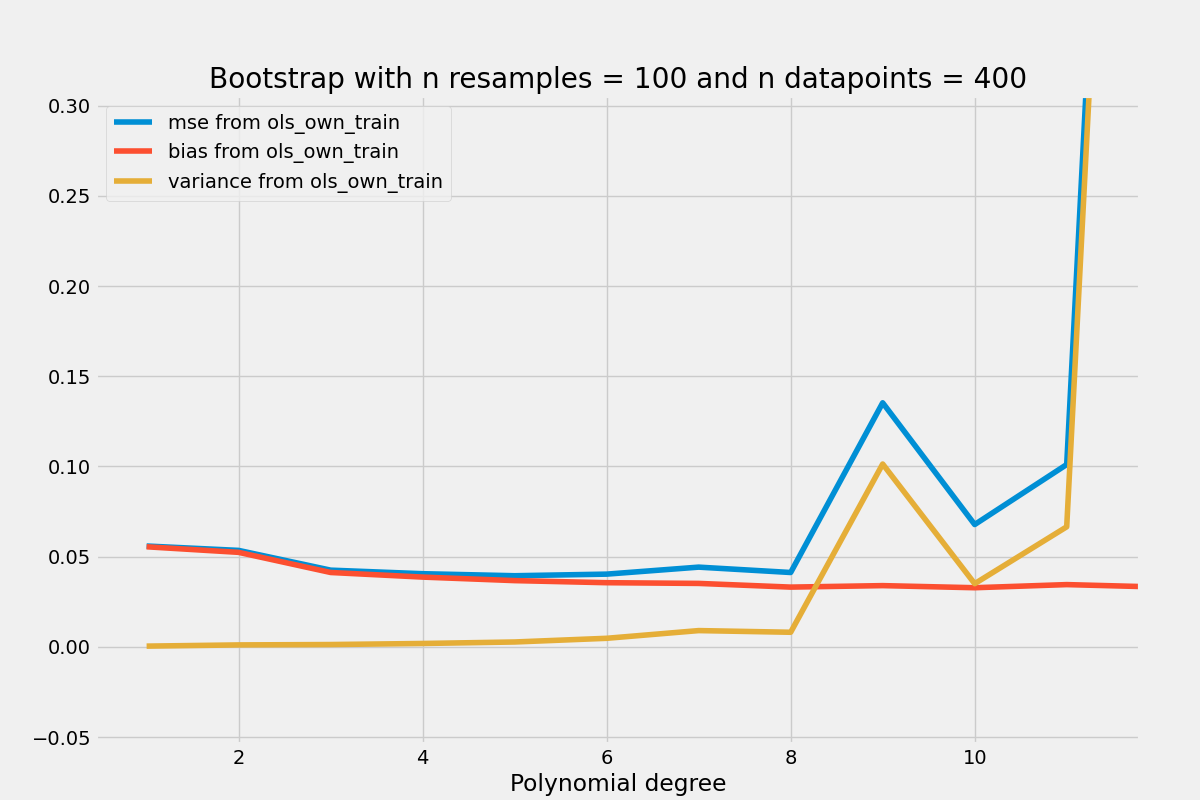
\includegraphics[width=0.8\textwidth]{Figures/c_bootstrap_ols_n_data_400_train_data.png}
    \caption{Bootstrap with 100 resamples for the OLS method on the Franke
    function on the training set with 400 datapoints.}
    \label{fig:bootstrap_ols_franke_train}
\end{figure}

Until now we have discussed our models in terms of MSE. However MSE is clolsy
related to bias and variance (see eq. \eqref{eq:bias_variance_decomposition}).
The variance describes the precision on our predicted models. As our model
complexity increases, it will be able to pick up complex patterns in our
training data. If we use another training dataset this pattern may not be
contained in the data. Thus our complex model fit will give different results.
If our models gets to complex it will describe patters that are unique to the
training data and not the representative distribution. This is called
over fitting and can be observed when the variance term rapidly increases with
model complexity. We previous saw that the MSE rapidly increases after a
certain polynomial. The reason is that the variance of the model increses, as
seen in figure \ref{fig:bootstrap_ols_franke_test} b and
\ref{fig:bootstrap_ols_franke_train}. 

The bias term is expected to go to zero as the model complexity increases. That
is our expected value of our models is approaching the real function. In our
results the bias term is decreasing (see fig \ref{fig:bootstrap_ols_franke_test} b and
\ref{fig:bootstrap_ols_franke_train}), as expected. But after a certain
polynomial degree the bias term is slightly increseing. This is somewhat
unexpected. However this may be due to the fact that the variance is
increseing and it's harder to obtain a good statistic on the real expectation
value of our model. This may have been resolved by increasing the number of
bootstrap re samples. It's also worth metntioning that we did not used the
exact function f(x) to esitamte the bias term. We used out test data, $\bm{y}
_{test} $. That is our exact function (Franke function) plus added normal
distributed noise. 
% This is probably why the bias term does not behave as
% expected. The statistics on our model (Expectation value) 
% TODO: think more





% To check the speculation of overfitting on the lower number of datapoints we
% look at figure \ref{fig:bootstrap_ols_franke_train} and we see here that the
% variance shoots off as the polynomial degree gets to 12. 

%%%%%%%%%%%%%%% Part d %%%%%%%%%%%%%%%
% Use k-fold and evaluate MEE on test data
% compare with bootstrap
% compare with sklearn


\begin{figure}[H]
    \centering
    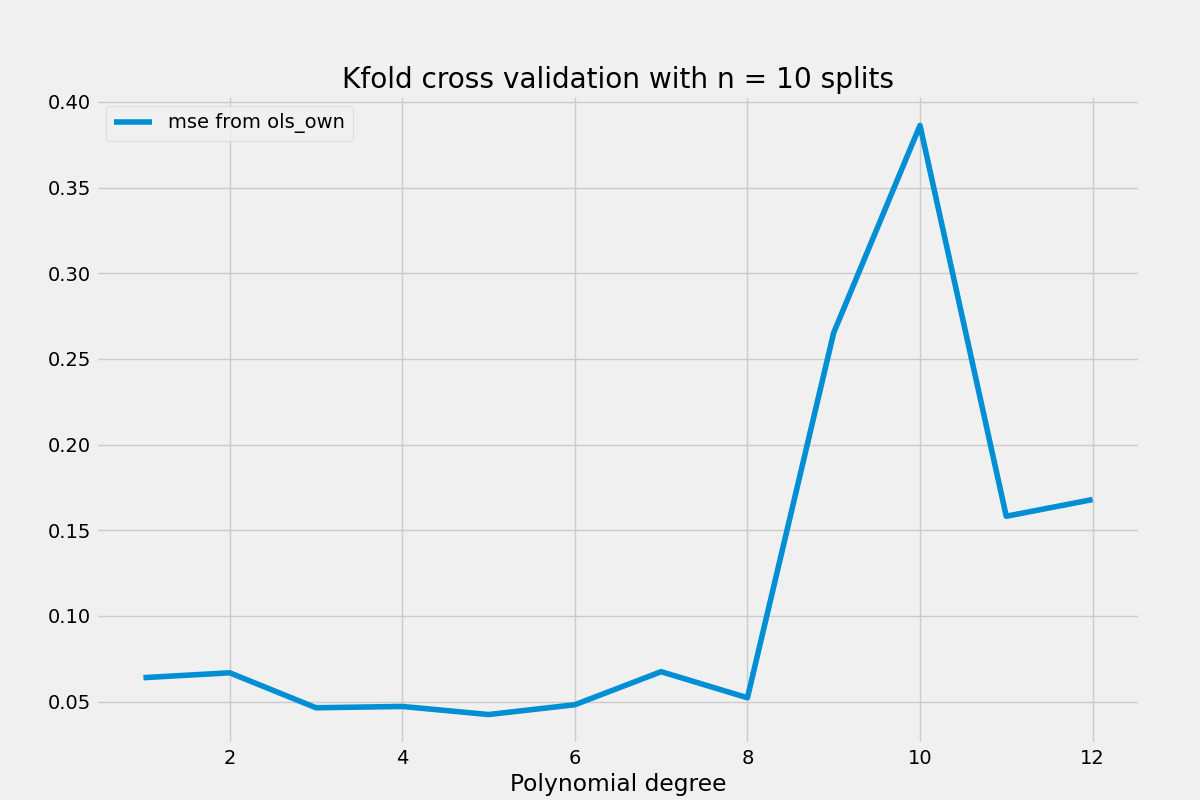
\includegraphics[width=0.8\textwidth]{Figures/d_kfold_ols_n_10.png}
    \caption{Mean squared error using cross-Validation with 10 splits on the Franke function.}
    \label{fig:kfold_ols_franke}
\end{figure}

In figure \ref{fig:kfold_ols_franke} we can see the MSE of Cross-validation with 10 spilts on the Franke function using OLS. This is on the test data. We see that polynomial degree over 8 produces weird results. This can be because of overfitting. 

%%%%%%%%%%%%%%% Part e %%%%%%%%%%%%%%%
% * bootstrap analysis for ridge as in part c
% * and cross validation as in part d 
% * Compare results to those obtained in part b-d
% * study bias variance trade off for different values of lambda 

The minimum MSE from Ridge regression was found for polynomial degree of 6 with
the hyper parameter, $\lambda = 0.001$. This is seen in figure \ref{fig:ridge_blabla}. Here we are to low in polynomial degree to see the typical bias-variance pattern.

\begin{figure}[H]
    \centering
    \caption{Ridge resgression on the Franke function.}
    \label{fig:ridge_blabla}
    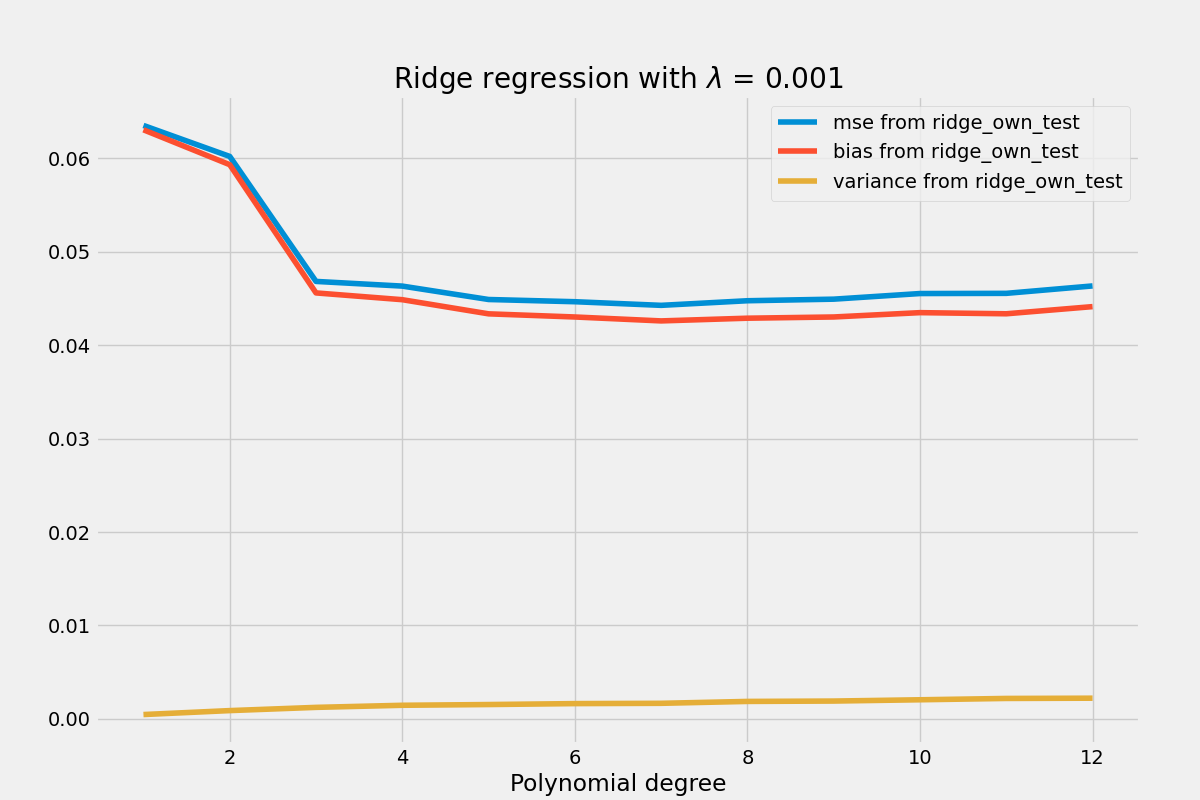
\includegraphics[width=0.8\textwidth]{Figures/e_ridge_bias_variance_lamb_0_001.png}
\end{figure}


\begin{figure}[H]
    \centering
    \caption{Correlation between MSE, the hyperparameter $\lambda$ and polyonmial degree for bootstrap on Ridge for on the Franke function.}  
    \label{fig:e_ridge} 
    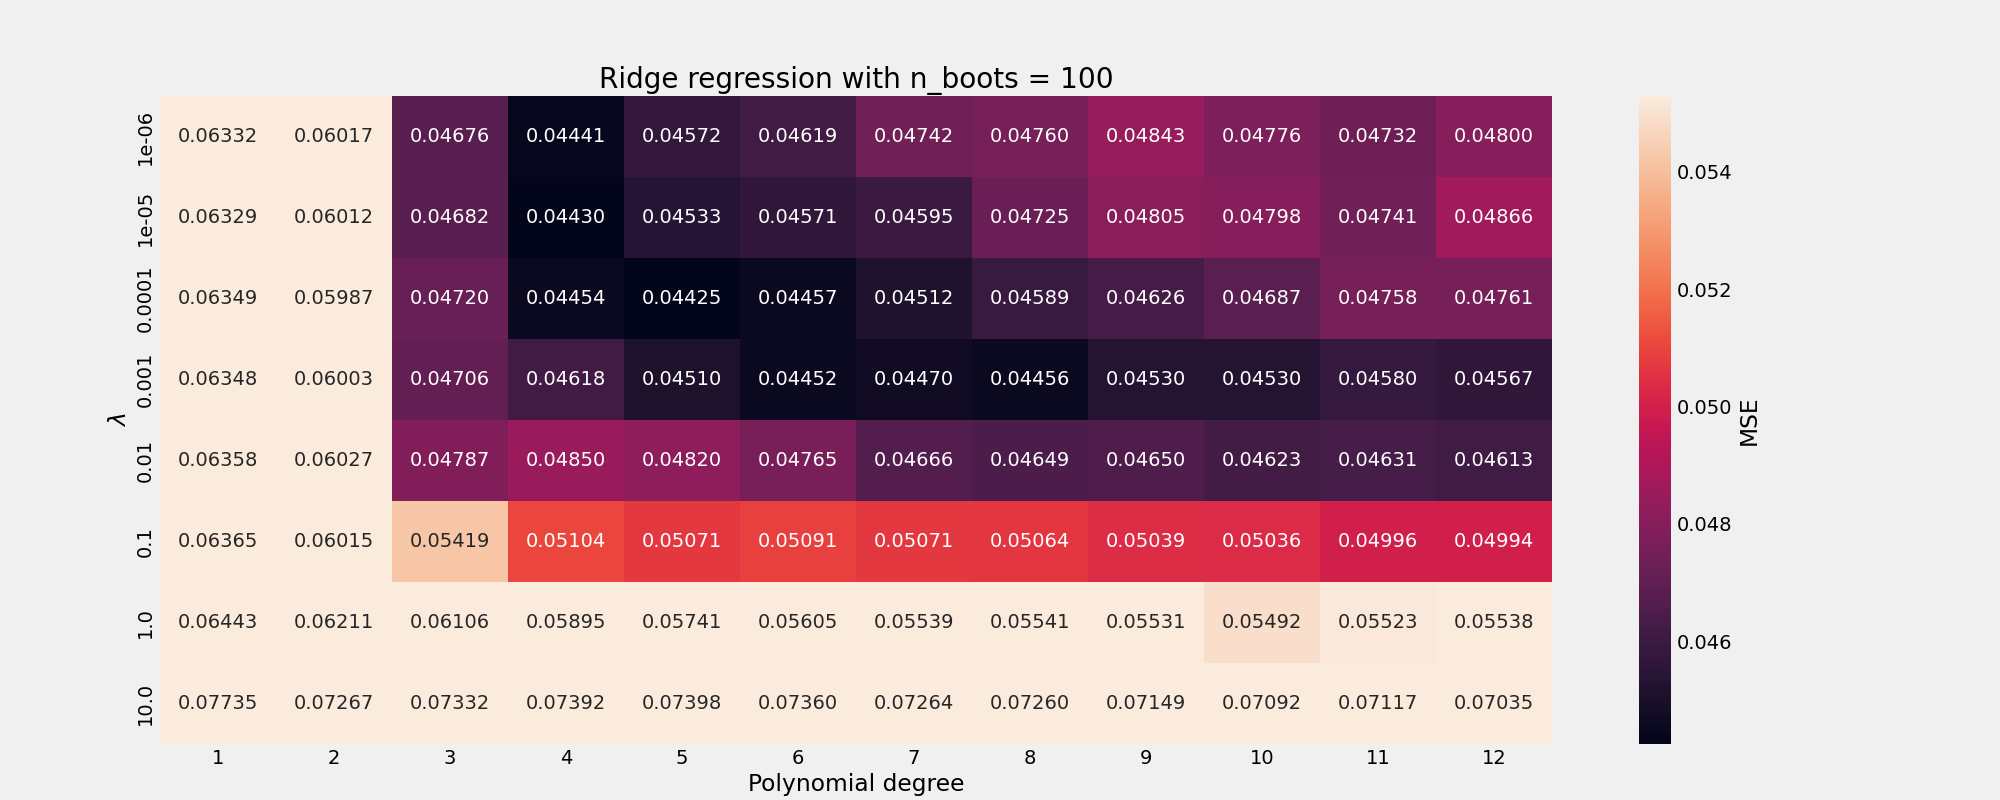
\includegraphics[width=1\textwidth]{Figures/e_ridge_n_boots_100.png}
\end{figure}

\begin{figure}[H]
    \centering
    \caption{Correlation between MSE, the hyperparameter $\lambda$ and polyonmial degree for Cross-Valdidation for Ridge regression on the Franke function.}
    \label{fig:e_ridge_kfold}
    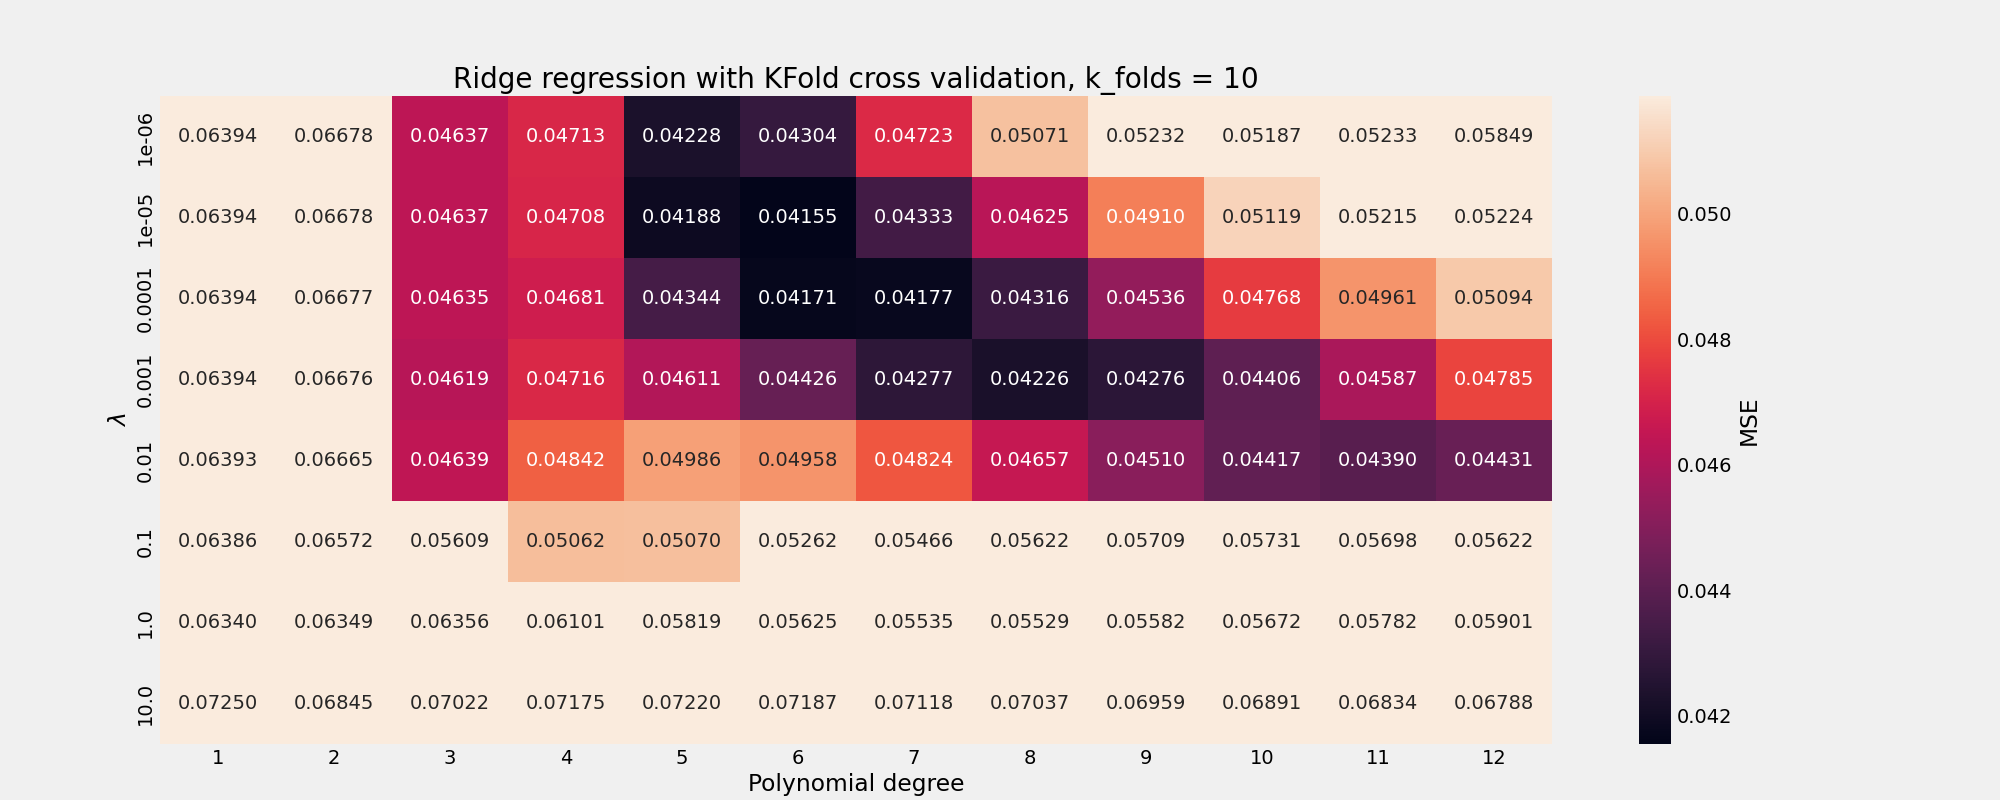
\includegraphics[width=0.8\textwidth]{Figures/e_ridge_kfold_n_10.png}
\end{figure}

Now we want to find the optimal $\lambda$ parameter 


%%%%%%%%%%%%%%% Part f %%%%%%%%%%%%%%%
% * Lasso regression
% * give a critical discussion of mse, ridge, lasso, in theory I discussed benefits of methods.
% * Which model fits the data best 
% * bootstrap bias variance analysis of lasso
% * MSE analysis with kfold


\begin{figure}[H]
    \centering
	\caption{Correlation between MSE, the hyperparameter $\lambda$ and polyonmial degree for Cross-Valdidation for Lasso regression on the Franke function.}
	\label{fig:f_lasso_bootstrap}
    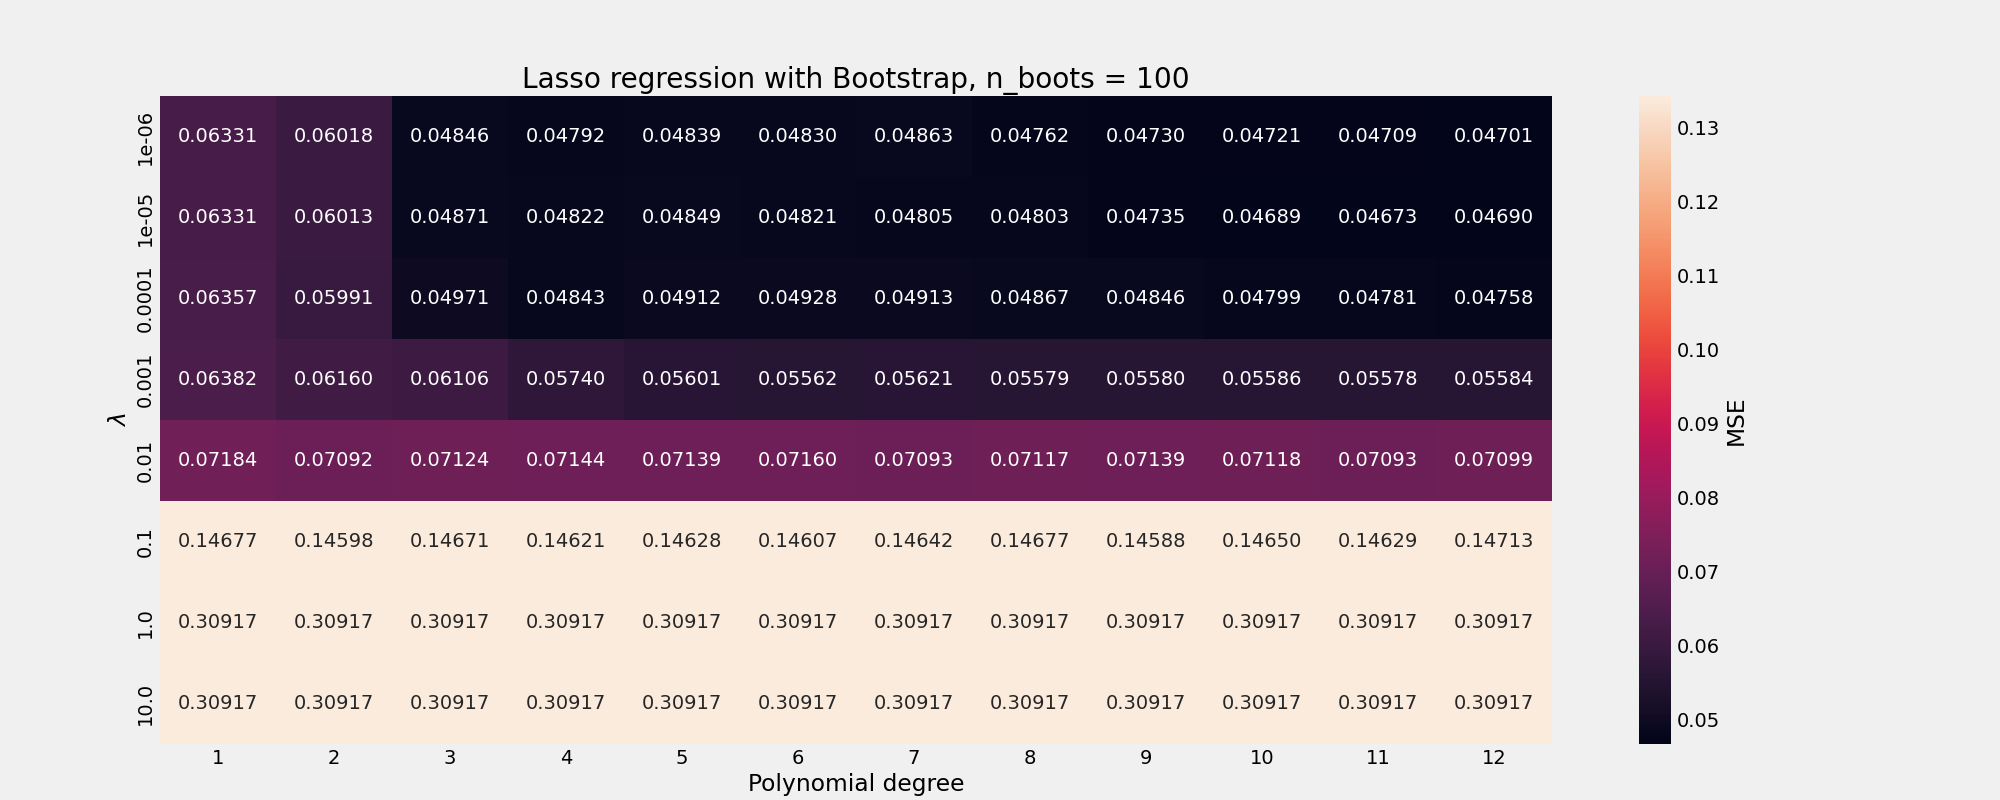
\includegraphics[width=0.8\textwidth]{Figures/f_lasso_bootstrap_n_100.png}
\end{figure}

\begin{figure}[H]
	\caption{Correlation between MSE, the hyperparameter $\lambda$ and polyonmial degree for Cross-Valdidation for Lasso regression on the Franke function.}
	\label{fig:f_lasso_kflod}
    \centering
    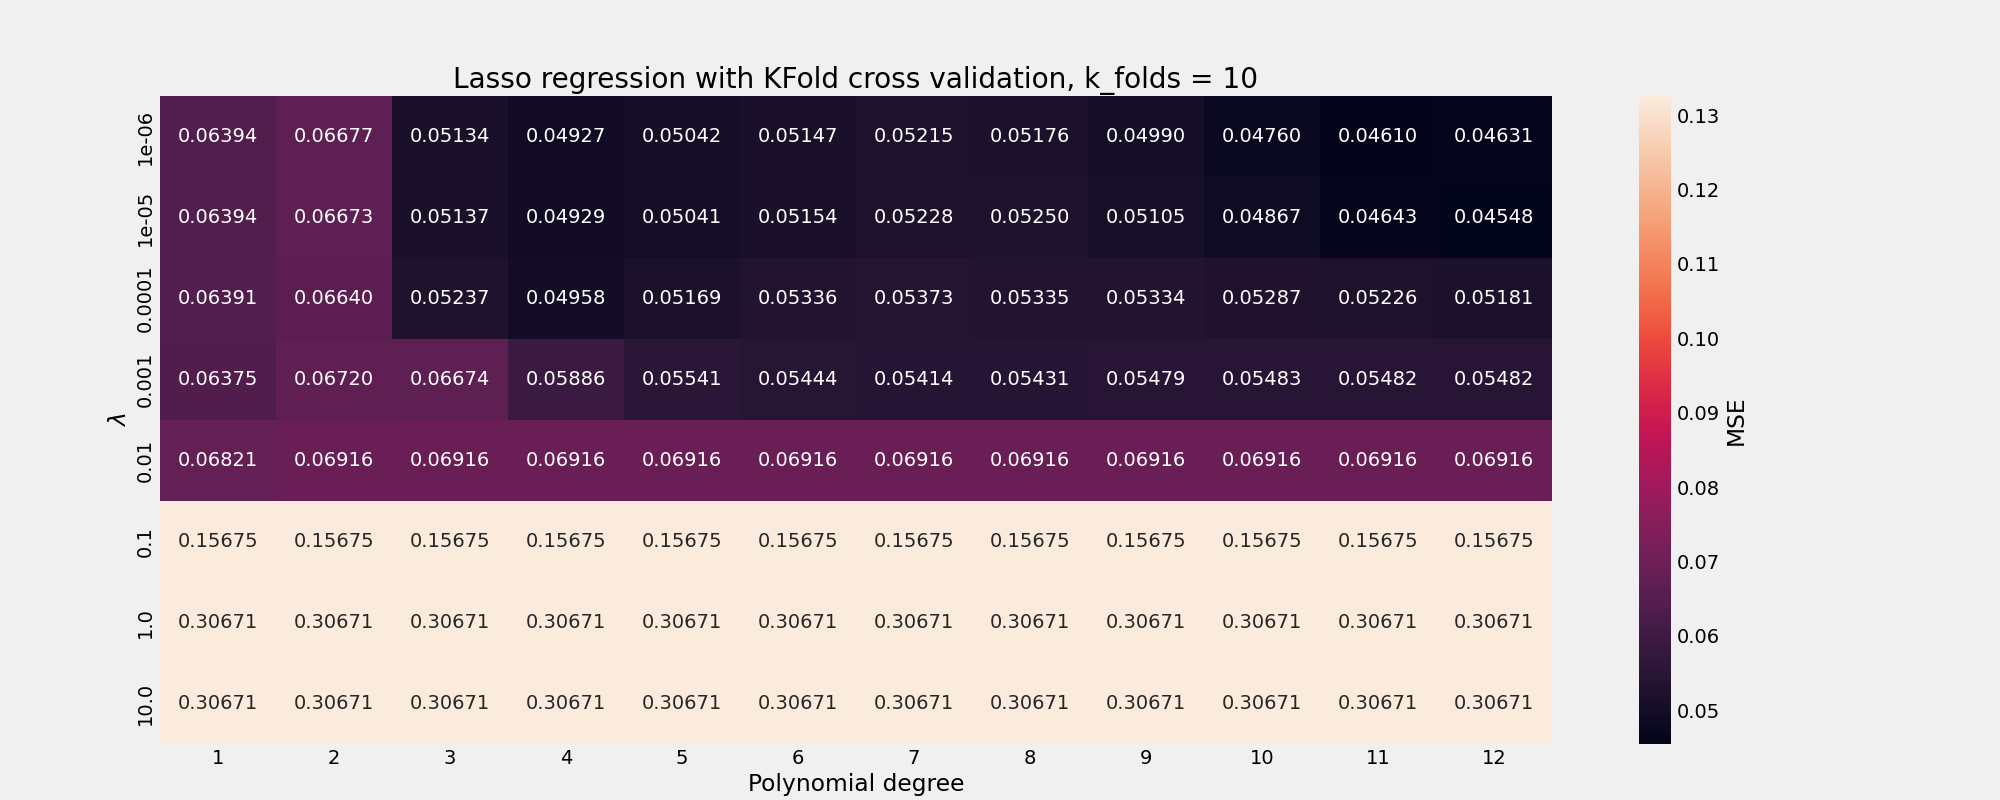
\includegraphics[width=0.8\textwidth]{Figures/f_lasso_kfold_n_10.png}
\end{figure}



% TODO: comparison of MSE for all methods
 
 %Maybe split results into two parts, Franke and Terrain data

%According to red line in report we want:
%On Franke-Function
%Subplot of MSE and R^2, test and training data, for OLS
%Subplot of MSE and R^2, test and training data, for Lasso
%Subplot of MSE and R^2, test and training data, for Ridge
%Comparrison of Regression methods
%Beta plot, but how to do this nicely, to show how beta values get large when polynomial degree increases.
%Resampling: bias-variance plot of bootstrap and cross-validation
%Study lambda dependence (correlation plot)

%On Terrain-data
%Subplot of MSE and R^2, test and training data, for OLS
%Subplot of MSE and R^2, test and training data, for Lasso
%Subplot of MSE and R^2, test and training data, for Ridge
%Comparrison of Regression methods
%Resampling: bias-variance plot of bootstrap and cross-validation
%Study lambda dependence (correlation plot)

%For critical discussion of centering/scaling, from lecture notes: "If our predictors represent different scales, then it is important to standardize the design matrix  by subtracting the mean of each column from the corresponding column and dividing the column with its standard deviation."




%%%%%%%%%%%%%%%%%%%%%%%%%%%%%%%%%%%%%%%%%%%%%
\subsection{Terrain data}
\begin{figure}[H]
    \centering
    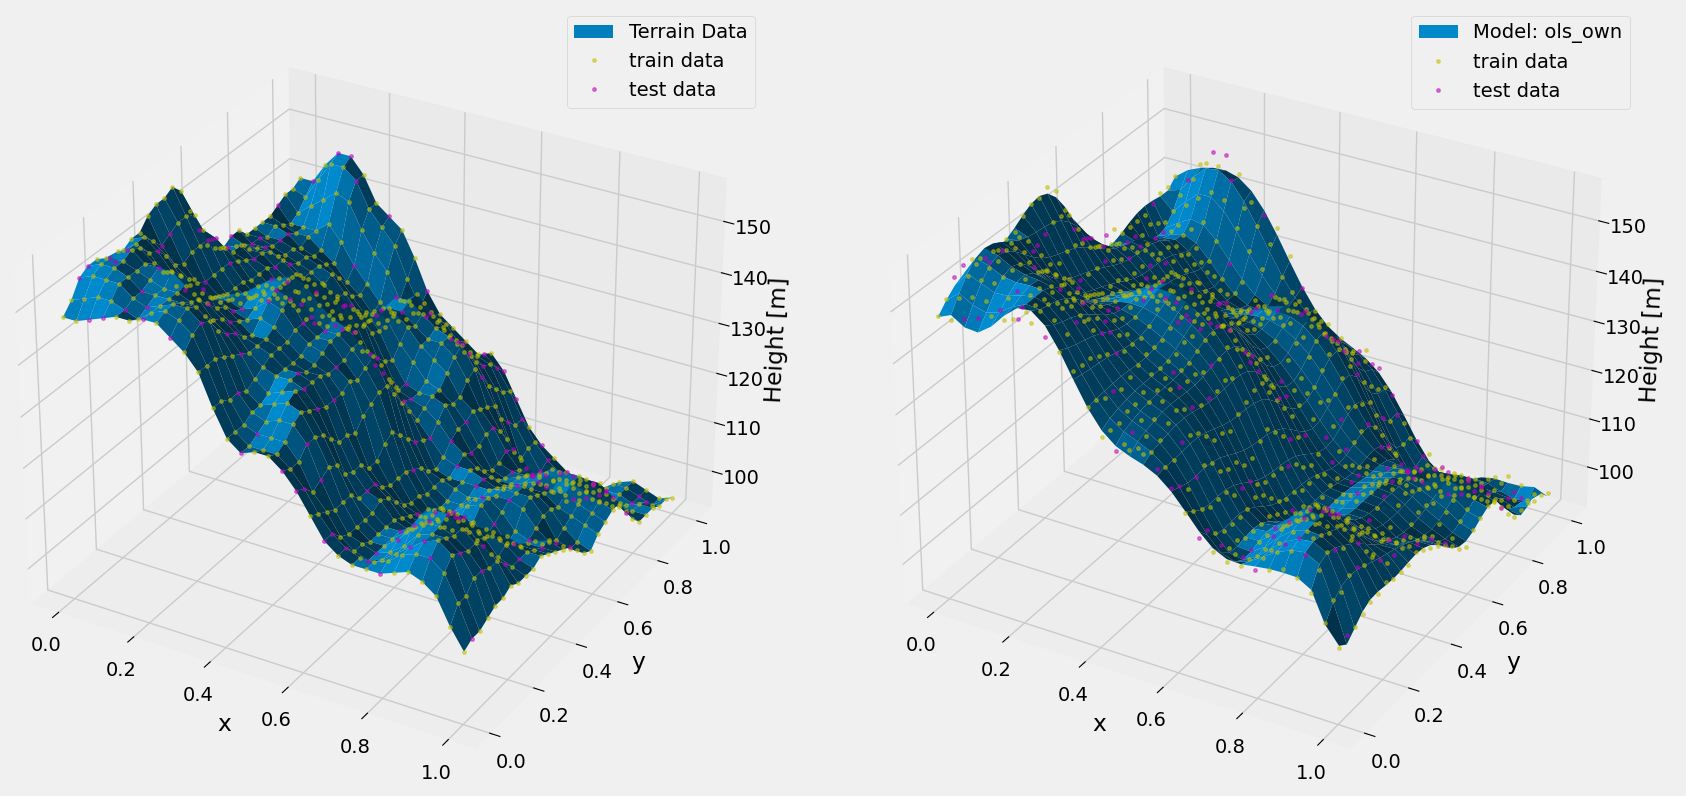
\includegraphics[width=0.8\textwidth]{Figures/terrain_data_and_model_ols_best.png}
    \caption{The left figure shows the surface of our sliced terrain data. Our
    train and test-data are represented by yellow and purple dots respectively.
Hight above sea level in meters is plotted on the z axis. The x- and y-axis is
takes values in intervall [0, 1]. This interval scales to 30m in real
coordinates. The left figure shows our best fit model obtained with OLS for
polynomial degree 18. Again the training- and test-data is plotted as in the
left figure.}  
\end{figure}

\begin{figure}[H]
    \centering
    \begin{subfigure}[b]{0.49\textwidth}
        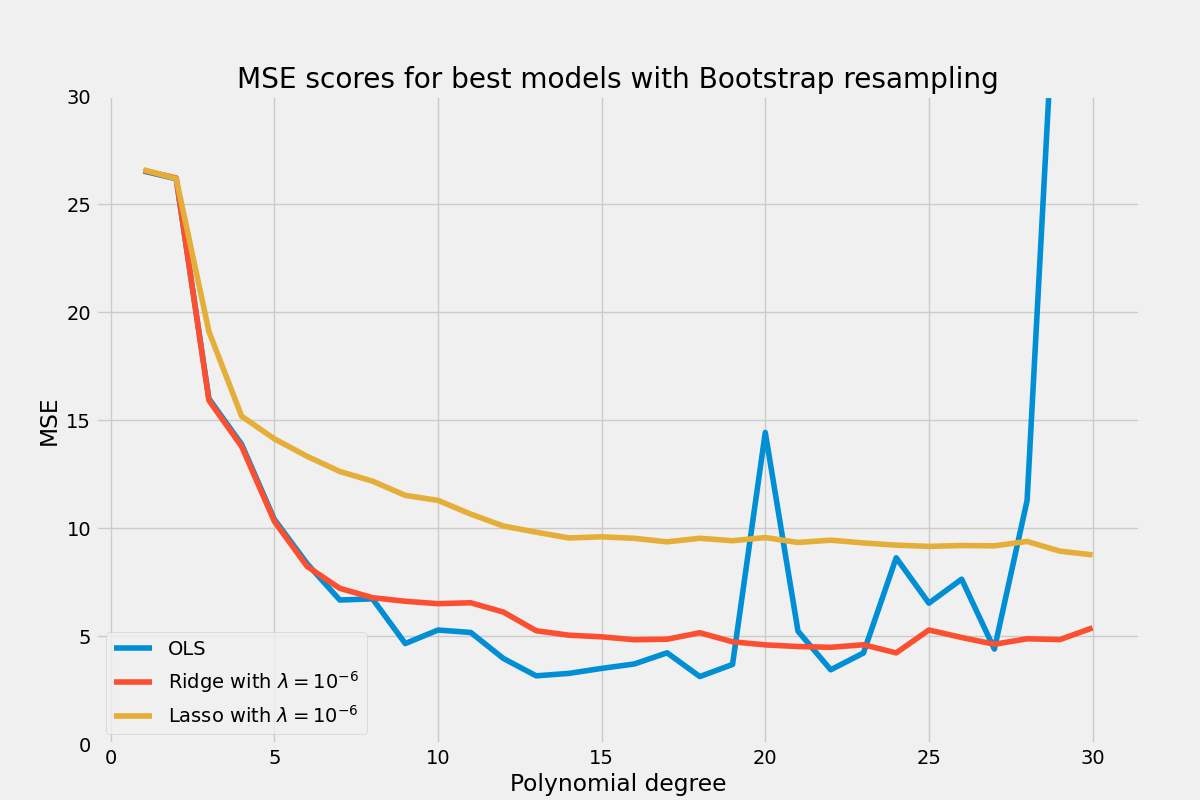
\includegraphics[width=\textwidth]{Figures/terrain_best_ols_ridge_lasso_boots.png}
        \caption{Mean of MSE scores calculated with bootstrap on the terrain data.\\ $n_{\text{boots}} =
        20$ re-samples was used. The mean MSE predicted on the test-data is plotted as
    function of polynomial degree for OLS-, Ridge- ($\lambda = 10^{6}$) and
Lasso-regression ($\lambda = 10^{-6})$   }  
    \end{subfigure}
    \begin{subfigure}[b]{0.49\textwidth}
        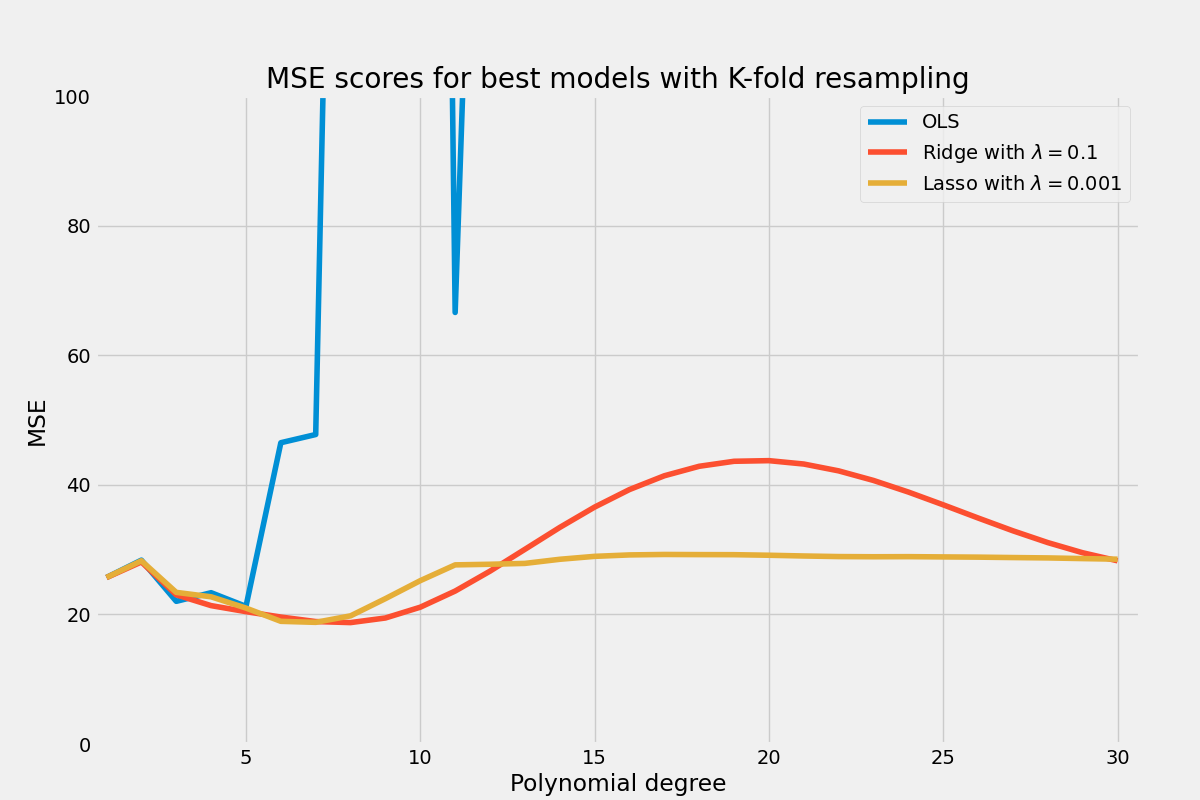
\includegraphics[width=\textwidth]{Figures/terrain_best_ols_ridge_lasso_kfold.png}
        \caption{Mean of MSE predicted on each test fold with use of the K-fold
        re-sampling technique. A total of ten folds was used. The MSE score is plotted as a function
    of polynomial degree for OLS-, Ridge- ($\lambda = 0.1$) and Lasso-regression
($\lambda = 10^{-4}$)}  
    \end{subfigure}
\end{figure}



\begin{figure}
\centering
\begin{subfigure}{0.49\textwidth}
    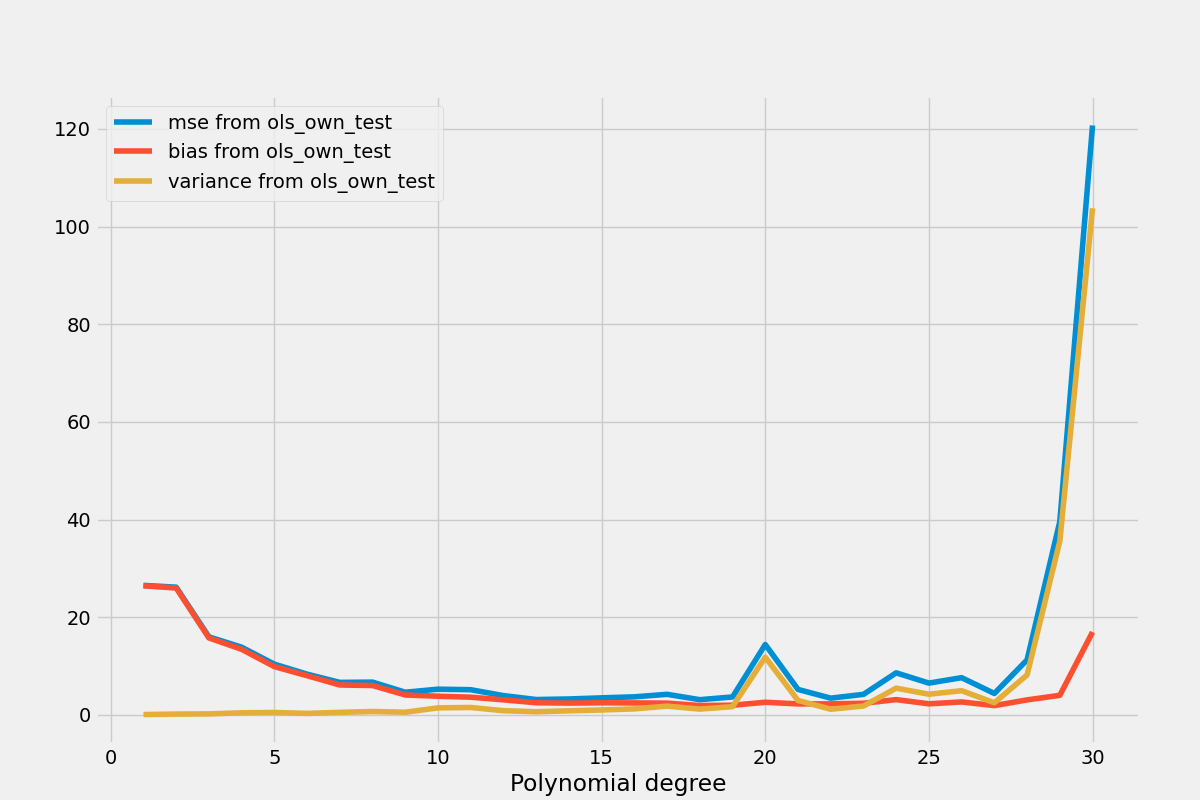
\includegraphics[width=\textwidth]{Figures/g_ols_bias_variance_boots_n_20.png}
    \caption{Bias, Variancse and MSE obtained with OLS and bootstrap re-sampling.
    20 re-samples was used to calculate the mean scores.}
    \label{fig:g_ols_bias_variance_boots}
\end{subfigure}
\hfill
\begin{subfigure}{0.49\textwidth}
    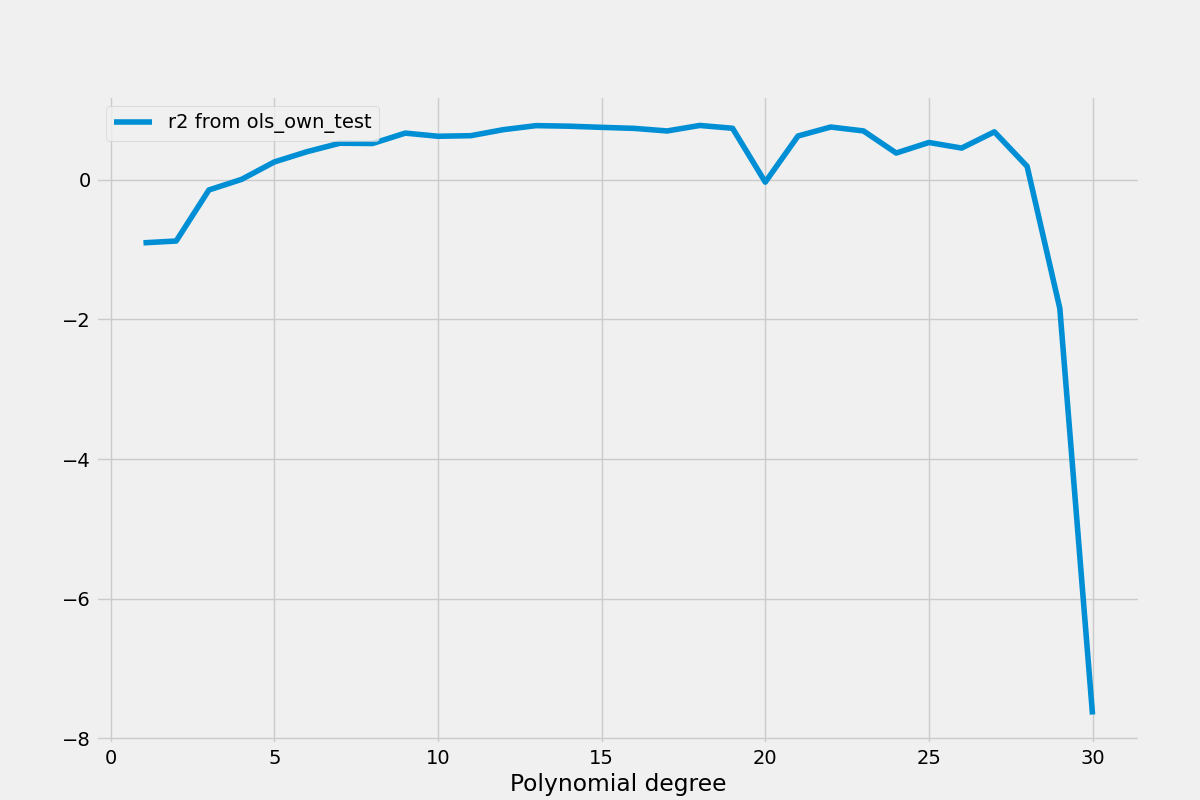
\includegraphics[width=\textwidth]{Figures/g_ols_r2_boots_n_20.png}
    \caption{R2 score obtained with OLS and bootstrap re-sampling.
    20 re-samples was used to calculate the mean R2 score.}
    \label{fig:g_ols_bias_variance_boots}
\end{subfigure}
\label{fig:g_ols_sub_plot}
\end{figure}

In figure \ref{fig:g_ols_sub_plot} we can see the score function and bias-variance plot for the OLS method using bootstrapping with 20 re-samples on the terrain data.

\begin{figure}[H]
    \centering
    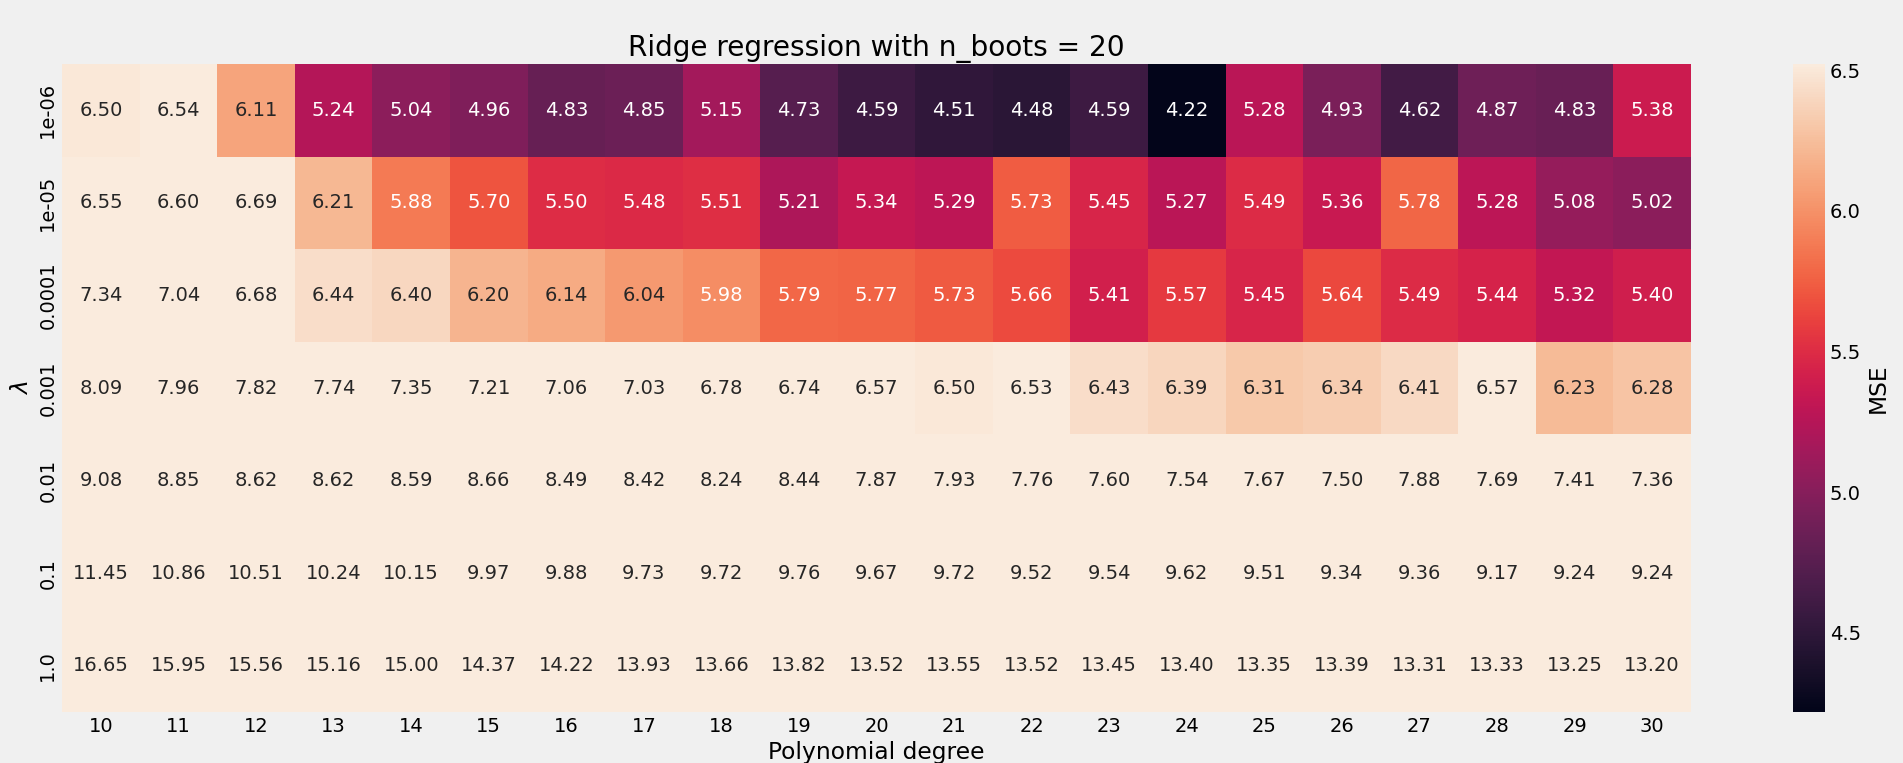
\includegraphics[width=\textwidth]{Figures/g_ridge_heatmap_boots_n_20.png}
    \caption{Heatmap of MSE scores obtained with Ridge regression and Bootstrap
    re-sampling, with 20 bootstrap re-sampling iterations.}  
    \label{fig:g_ridge_boost_heatmap}  
\end{figure}

\begin{figure}[H]
    \centering
    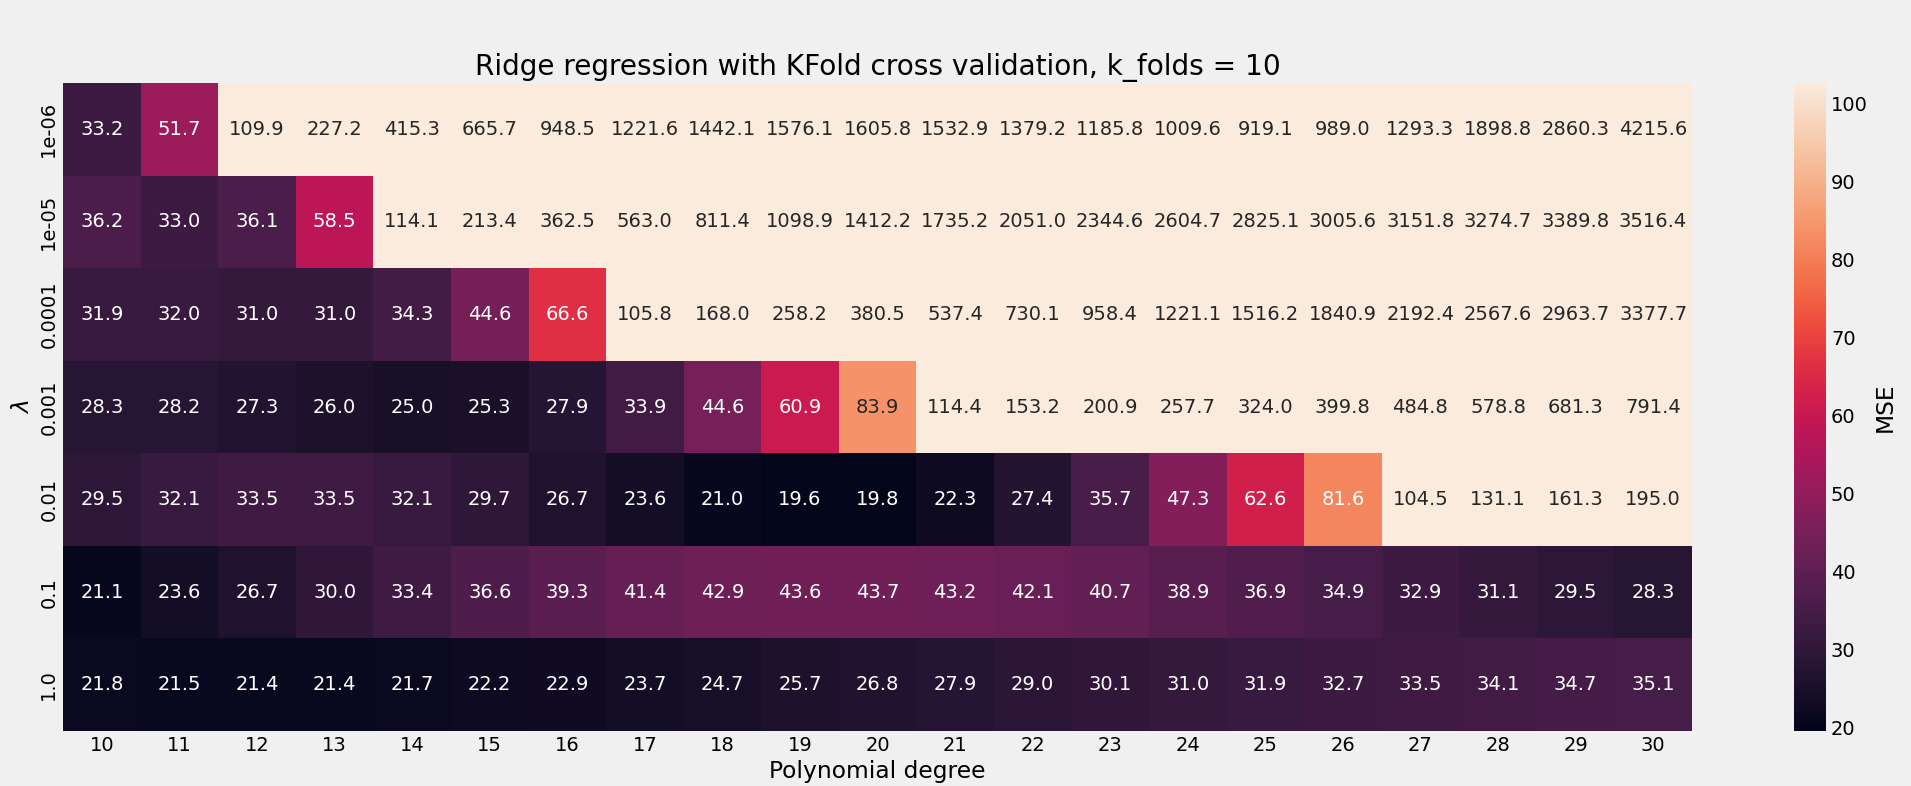
\includegraphics[width=\textwidth]{Figures/g_ridge_heatmap_kfold_n_10.png}
    \caption{Heatmap of MSE scores obtained with Ridge regression and K-fold
    re-sampling, with 10 splits.}  
    \label{fig:g_ridge_kfold_heatmap}  
\end{figure}

\begin{figure}[H]
    \centering
    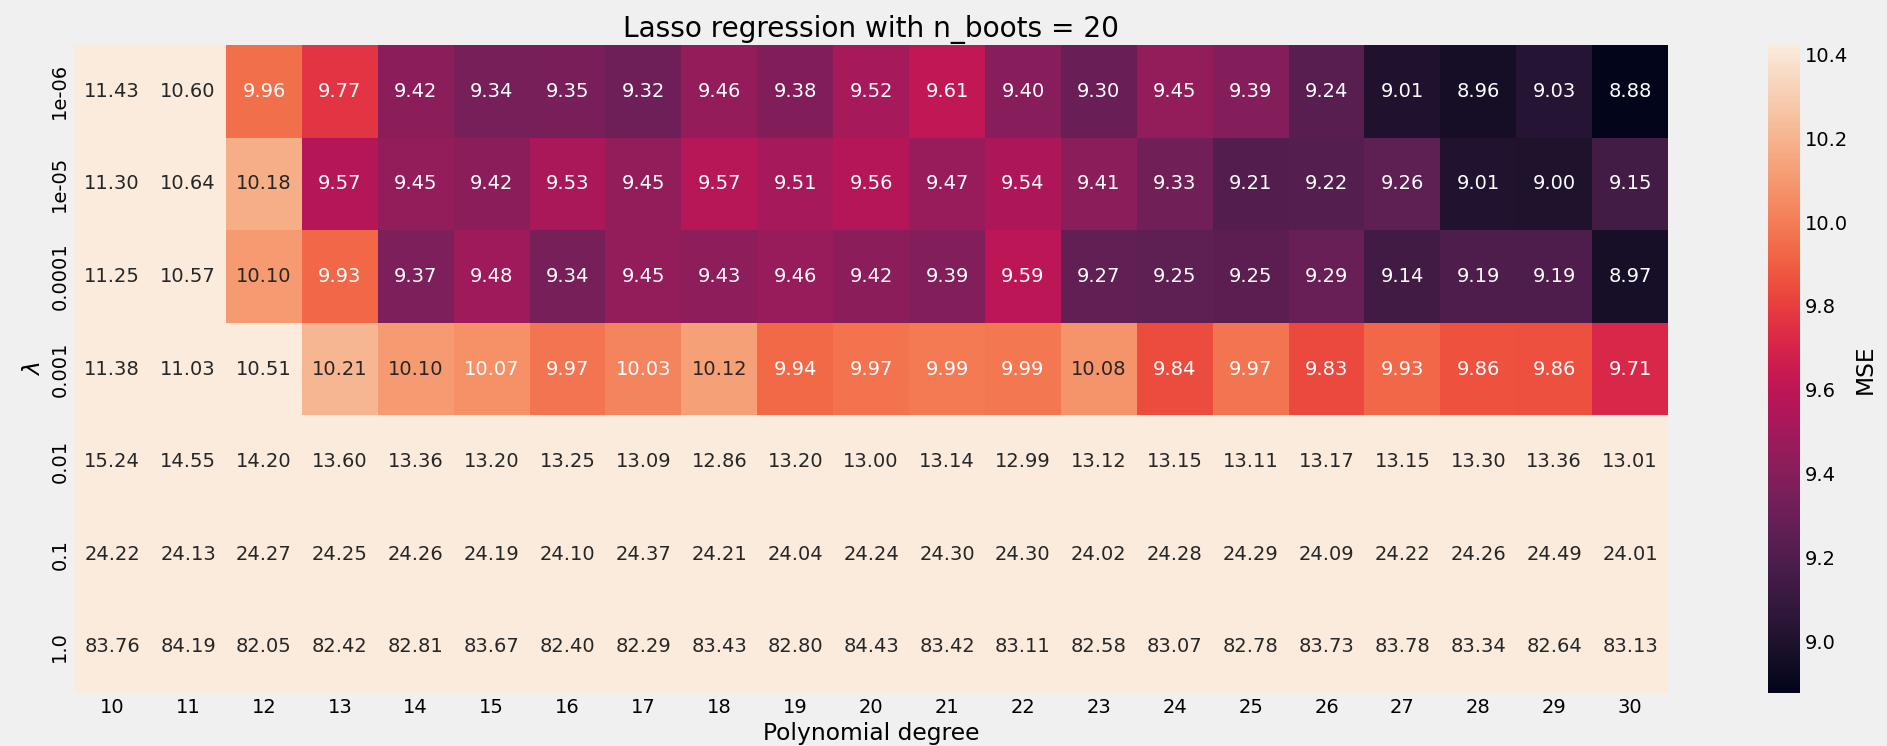
\includegraphics[width=\textwidth]{Figures/g_lasso_heatmap_boost_n_20.png}
    \caption{Heatmap of MSE scores obtained with lasso regression and Bootstrap
    re-sampling, with 20 re-samples.}  
    \label{fig:g_lasso_boots_heatmap}  
\end{figure}

\begin{figure}[H]
    \centering
    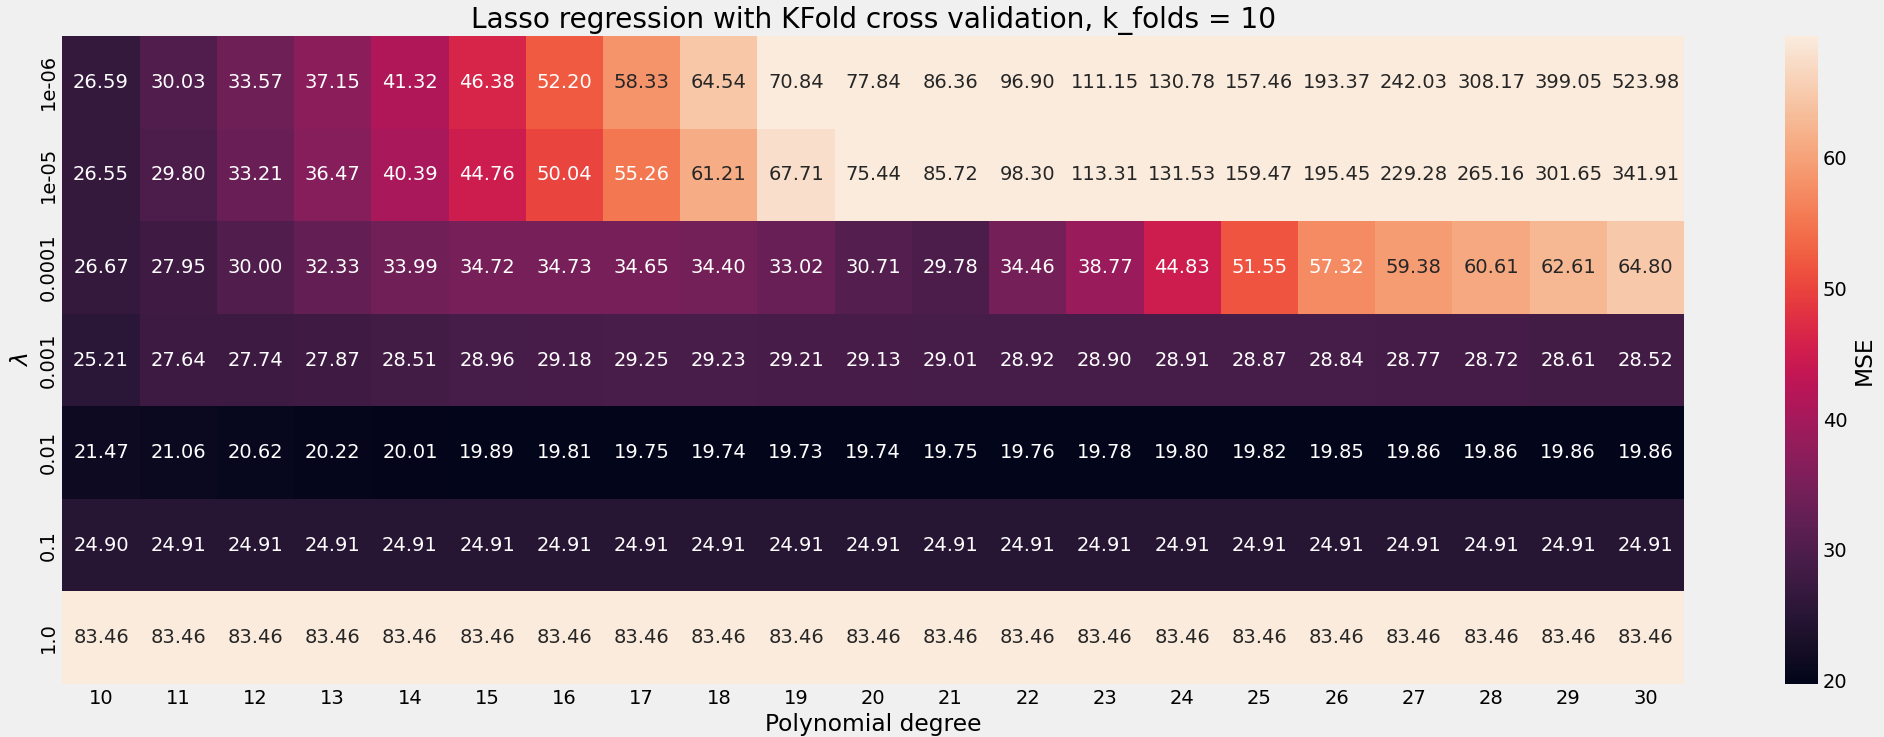
\includegraphics[width=\textwidth]{Figures/g_lasso_heatmap_kfold_n_10.png}
    \caption{Heatmap of MSE scores obtained with lasso regression and K-fold
    re-sampling, with 10 splits.}  
    \label{fig:g_lasso_boots_heatmap}  
\end{figure}

In figure \ref{fig:g_ridge_boost_heatmap}, \ref{fig:g_ridge_kfold_heatmap}, \ref{fig:g_lasso_boots_heatmap} and \ref{fig:g_lasso_boots_heatmap} we see the MSE for a number of polynomial degreees and $\lambda$'s on the terrain data function. We notice that for Lasso a bigger $\lambda$ tend to provide smaller MSE, while for Ridge it's the opposite. This means the OLS method and the Ridge method would produce similar results. 

\begin{table}
    \centering
    \caption{Table of Best mean squared error (MSE) scores obtained with
        different re-sampling and regression
        methods. $\lambda $ is the best choice of regularization parameters for
        Ridge and Lasso regression. n refers to number of re-samples/splits used in
        Bootstrap and K-fold.}  
    \label{tab:terrain_mse_best} 
    \begin{tabular}{|c|c|c|c|c|}
        \hline
        Polynomial degree & $\lambda$ & Regression method & Re-sampling method & MSE \\
        \hline
                          18 &   &  OLS & Bootstrap (n=20) & 3.12\\
        \hline

                          24 & $10^{-6}$ &   Ridge & Bootstrap (n=20) & 4.22\\
        \hline

                          30 &  $10^{-6}$ & Lasso&  Bootstrap (n=20) & 8.88\\
        \hline

                          5 &  & OLS & K-fold (n=10)& 21.23\\
        \hline

                          8 &  0.1 & Ridge & K-fold (n=10)& 18.74\\ % XXX: new - forgot to inspect deg 0-10
                          % 19 &  0.01 & Ridge & K-fold (n=10)& 19.6  XXX: old
        \hline
                          7 & 0.001 &  Lasso & K-fold (n=10)& 18.77\\ % XXX: new
                          % 19 & 0.01 &  Lasso & K-fold (n=10)& 19.73\\ % XXX: old
        \hline
    \end{tabular} 
\end{table}

We see in table \ref{tab:terrain_mse_best} that the optimal polynomial degrees are higher for Ridge and Lasso both with bootstrap and Cross-Validation.



\begin{figure}[H]
    \centering
	\label{fig:g_ols_ridge_lasso_boots}
	\caption{Mean squared error as a function of polynomial degree for the regression methods OLS, Ridge and Lasso using ? number of bootstraps on the terrain data.}
    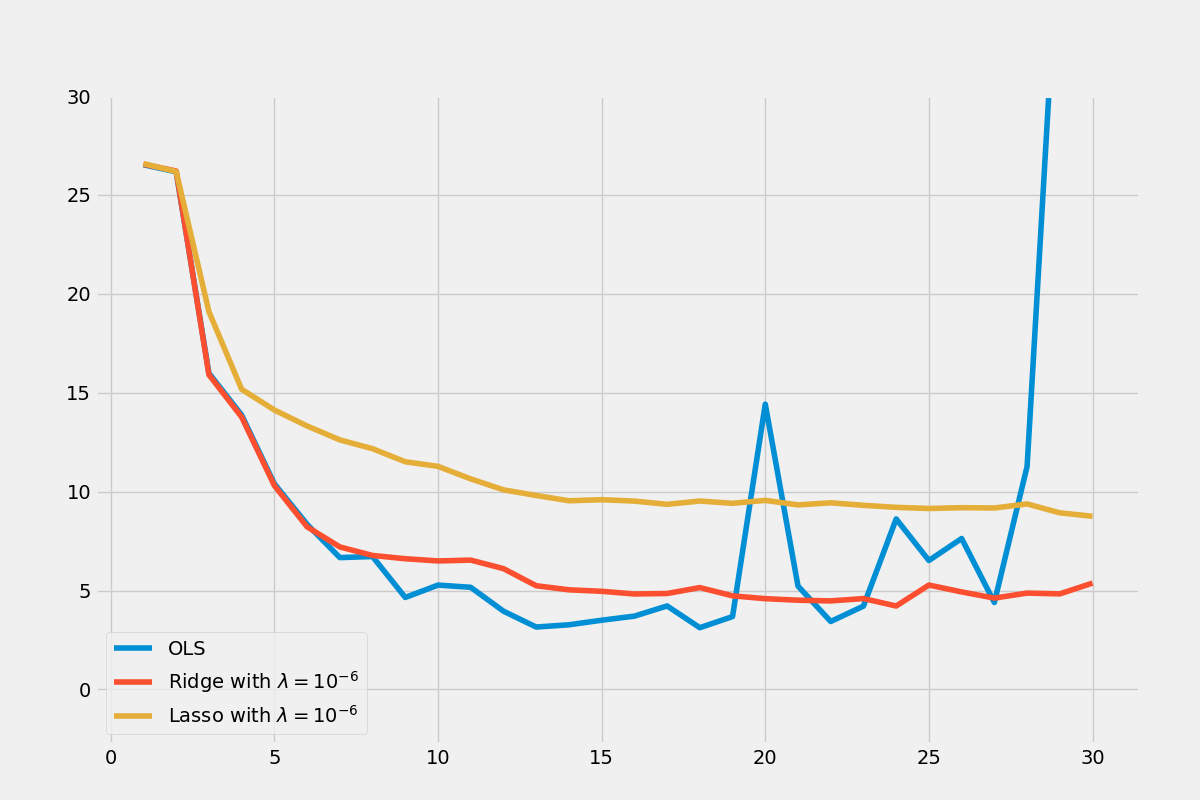
\includegraphics[width=0.8\textwidth]{Figures/g_ols_ridge_lasso_boots_n_20.png}
\end{figure}

In figure \ref{fig:g_ols_ridge_lasso_boots} we can see the MSE for the three different regression methods. We see that Lasso and Ridge regression is more stable but OLS beats both methods at around polynomial degree 12. But then we see overfitting of the OLS method at higher degree polynomials.



